\documentclass[notheorems]{beamer}
% \documentclass{beamer}

\mode<presentation>
{
  % \usetheme{default}
  \usetheme{Antibes}
  \setbeamertemplate{footline}[frame number]{}
  \setbeamertemplate{navigation symbols}{}
}

\usepackage{amsmath}
\usepackage{ragged2e}
\usepackage{yhmath}

\justifying\let\raggedright\justifying

\makeatletter
\newenvironment<>{proofs}[1][\proofname]{
    \par
    \def\insertproofname{#1\@addpunct{.}}
    \usebeamertemplate{proof begin}#2}
  {\usebeamertemplate{proof end}}

  \newenvironment<>{solution}[1][Solution.]{
    \par
    \def\insertproofname{#1\@addpunct{.}}
    \usebeamertemplate{proof begin}#2}
  {\usebeamertemplate{proof end}}

  \newtheorem*{definition}{Definition}
  \newtheorem{example}{Example}[section]
  \newtheorem{theorem}{Theorem}[section]
  \newtheorem{property}{Property}[section]
\makeatother

\setbeamertemplate{theorems}[numbered]
% \setbeamertemplate{definition}[nonumbered]

\setbeamertemplate{section in toc}[sections numbered]
\setbeamertemplate{subsection in toc}[subsections numbered]
% \setbeamertemplate{subsubsection in toc}[subsubsections numbered]

\numberwithin{equation}{section}
\numberwithin{equation}{subsection}

\usefonttheme[onlymath]{serif}
\providecommand{\Arg}{\operatorname{Arg}}
\providecommand{\Ln}{\operatorname{Ln}}
\providecommand{\Arcsin}{\operatorname{Arcsin}}
\providecommand{\Arccos}{\operatorname{Arccos}}
\providecommand{\Arctan}{\operatorname{Arctan}}
\providecommand{\Arcsinh}{\operatorname{Arcsinh}}
\providecommand{\Arccosh}{\operatorname{Arccosh}}
\providecommand{\Arctanh}{\operatorname{Arctanh}}
\DeclareMathOperator{\dif}{d \!}

% \providecommand{\abs}[1]{\lvert#1\rvert}
\providecommand{\abs}[1]{\left\lvert#1\right\rvert}
% \providecommand{\norm}[1]{\lVert#1\rVert}

\title{Chapter 3: Complex Integration}
\author{Taotao Wang, Associate Professor}
\institute{College of Electronics and Information Engineering, Shenzhen University}
% \date{\today}

\begin{document}

\everymath{\displaystyle}

\begin{frame}
  \titlepage
\end{frame}

\begin{frame}{Outline}
  \tableofcontents
\end{frame}

\section{Concept of Complex Integration}

\begin{frame}
  \frametitle{Outline}
  \tableofcontents[currentsection]
\end{frame}

\begin{frame}
	\begin{enumerate}
		\item \textbf{Definition of Complex Integration}
		\begin{enumerate}[1)]
			\item Directed Curve
		\end{enumerate}
	\end{enumerate}
	\begin{definition}
		Let $C$ be a given smooth (or piece-wise smooth) curve on the plane. If one of the two directions of $C$ is selected as the positive direction, $C$ is called a directed curve.
	\end{definition}
	\begin{minipage}[b]{0.6\linewidth}
		If $A$ to $B$ is the positive direction of curve $C$, then $B$ to $A$ is the negative direction of curve $C$, which is denoted by $C^-$.
	\end{minipage}
	\begin{minipage}{0.4\linewidth}
		\begin{figure}
			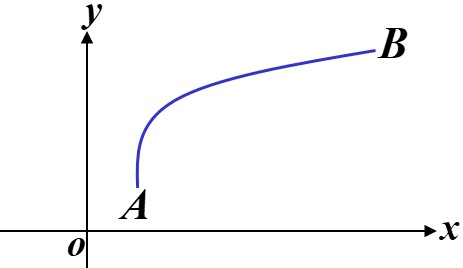
\includegraphics[width=\linewidth]{Figure_3_1_1.jpg}
		\end{figure}
	\end{minipage}
\end{frame}

\begin{frame}
  If the curve is a simple closed curve, it is usually specified that the counterclockwise direction is positive and the clockwise direction is negative. If the closed curve is used as the boundary of an domain, its positive direction is specified as:
  \vspace{\baselineskip}\\
  \begin{minipage}[c]{0.6\linewidth}
    When we take a point $P$ on the closed curve and move the point $P$ on the curve along a direction, if the domain adjacent to point $P$ is always on the left side of the closed curve, we say that the direction is the positive direction of the closed curve.
  \end{minipage}
  \begin{minipage}[T]{0.4\linewidth}
    \begin{figure}
      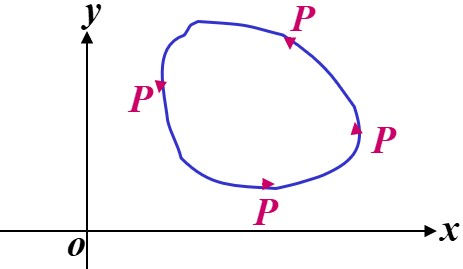
\includegraphics[width=\linewidth]{Figure_3_1_2.jpg}
    \end{figure}
  \end{minipage}
  \vspace{\baselineskip}\\
  Obviously, the positive direction of the outer boundary of a domain is counterclockwise, and the positive direction of the inner boundary of a domain is clockwise.
\end{frame}


\begin{frame}
	\setcounter{enumi}{2}
	\begin{enumerate}[2)]
        \item Definition of Complex Integration
	\end{enumerate}
	\begin{definition}
		Let the function $f(z)$ is defined in the domain $D$, $C$ is a smooth directed curve with a starting point of $A$ and an ending point of $B$ in $D$. The curve $C$ is arbitrarily divided into $n$ arc segments, and the dividing point is
		\[A=z_0,z_1,z_2,\cdots,z_{k-1},z_k,\cdots,z_n=B.\]
		We take a any point $\zeta_k$ on each arc segment $\wideparen{z_{k-1}z_k}$, $k=1,2,\cdots,n$ (see Figure 3.1) and make the following summation:
		\[S_n=\sum_{k=1}^{n}f(\zeta_k)(z_k-z_{k-1})=\sum_{k=1}^{n}f(\zeta_k)\Delta z_k,\]
		where $\Delta z_k=z_k-z_{k-1}$.
	\end{definition}
\end{frame}



\begin{frame}
	\begin{definition}[Cont.]
		Let $\Delta s_k$ be the length of arc segment $\wideparen{z_{k-1}z_k}$, $\delta=\max_{1\leq k\leq n}\{\Delta s_k\}$. When $n\to\infty$ and $\delta\to 0$, $S_n$ always has a unique limit regardless of the division of $C$ and the choice of $\zeta_k$. This limit value is called the integral of the function $f(z)$ along the curve $C$, which is denoted by\\
		\begin{minipage}[b]{0.55\linewidth}
			$\int_C f(z)\dif z=\lim_{n\to\infty}\sum_{k=1}^n f(\zeta_k)\Delta z_k$.
		\end{minipage}
		\begin{minipage}{0.4\linewidth}
			\begin{figure}
				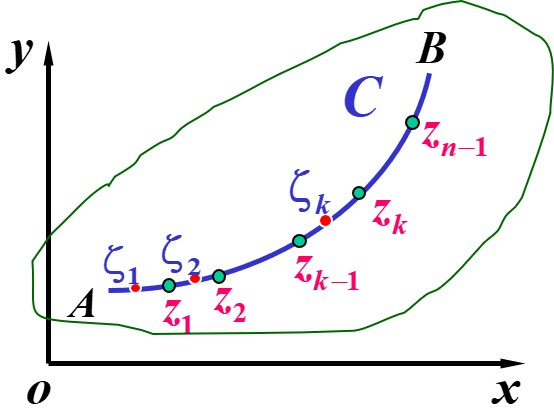
\includegraphics[width=\linewidth]{Figure_3_1_3.jpg}
			\end{figure}
		\end{minipage}
	\end{definition}
\end{frame}


\begin{frame}
	\begin{enumerate}
		\item []
		Discussions about the definition of complex integral:
		\begin{enumerate}[i)]
			\item If $C$ is a closed curve, the integral along this closed curve is written as $\oint f(z)\dif z$.
			\item If $C$ is the interval $a\leq x\leq b$ on the $x$-axis and $f(z)=u(x)$, the definition of this integral is the same as the definition of the definite integral of a real function with one variable.
		\end{enumerate}
	\end{enumerate}
\end{frame}

\begin{frame}
	\setcounter{enumi}{2}
	\begin{enumerate}[2]
		\item \textbf{Condition for the Existence of Integral and Its Calculation Method}
	\end{enumerate}
	\begin{theorem}[the existence of complex integral]
		If $f(z)=u(x,y)+iv(x,y)$ is continuous on smooth curve $C$ and $\int_C f(z)\dif z$ exists, then
		\[\int_C f(z)\dif z=\int_C u\dif x-v\dif y+i\int_C v\dif x+u\dif y.\]
	\end{theorem}
	\begin{proofs}[\proofname]<2->
		Let $z_k=x_k+iy_k$, $\zeta_k=\xi_k+i\eta_k$ and
		$\begin{aligned}
			\Delta z_k & =z_k-z_{k-1}=x_k+iy_k-(x_{k-1}+iy_{k-1}) \\
			& =(x_k-x_{k-1})+i(y_k-y_{k-1})            \\
			& =\Delta x_k+i\Delta y_k,
		\end{aligned}$
	\end{proofs}
\end{frame}

\begin{frame}
	\begin{proofs}[\proofname\ (Cont.)]
		So $\begin{aligned}[t]
			& \sum_{k=1}^n f(\zeta_k)\cdot\Delta z_k                                          \\
			= & \sum_{k=1}^n \big[u(\xi_k,\eta_k)+iv(\xi_k,\eta_k)\big](\Delta x_k+i\Delta y_k) \\
			= & \sum_{k=1}^n \big[u(\xi_k,\eta_k)\Delta x_k-v(\xi_k,\eta_k)\Delta y_k\big]      \\
			& +i\sum_{k=1}^n \big[v(\xi_k,\eta_k)\Delta x_k+u(\xi_k,\eta_k)\Delta y_k\big]
		\end{aligned}$
	\end{proofs}
\end{frame}

\begin{frame}
	\begin{proof}[\proofname\ (Cont.)]
		Since $u$ and $v$ are continuous functions, according to the existence theorem of line integral, when $n$ increases infinitely and the maximum value of arc length tends to zero, regardless of the division of $C$ and the selection of points $(\xi_k,\eta_k)$, the limits at both ends of the following formula exist.
		\begin{align*}
			{\color{red}\boxed{\color{black}\sum_{k=1}^n f(\zeta_k)\Delta z_k}}= & {\color{blue}\boxed{\color{black}\sum_{k=1}^n \big[u(\xi_k,\eta_k)\Delta x_k-v(\xi_k,\eta_k)\Delta y_k\big]}}         \\
			& +i{\color{green}\boxed{\color{black}\sum_{k=1}^n \big[v(\xi_k,\eta_k)\Delta x_k+u(\xi_k,\eta_k)\Delta y_k\big]}}      \\
			{\color{red}\boxed{\color{black}\int_C f(z)\dif z}}=                 & {\color{blue}\boxed{\color{black}\int_C u\dif x-v\dif y}}+i{\color{green}\boxed{\color{black}\int_C v\dif x+u\dif y}}
		\end{align*}
	\end{proof}
\end{frame}


\begin{frame}
	\begin{enumerate}
		\item []
		Note:
		\begin{enumerate}[i)]
			\item The right side of the above formula can be obtained by multiplying $f(z)=u+iv$ with $\dif z=\dif x+i\dif y$:
			\begin{align*}
				\int_C f(z)\dif z & =\int_C (u+iv)(\dif x+i\dif y)                 \\
				& =\int_C u\dif x+iv\dif x+iu\dif y-v\dif y      \\
				& =\int_C u\dif x-v\dif y+\int_C v\dif x+u\dif y
			\end{align*}
			\item If curve $C$ is given by parametric equation $z=z(t)=x(t)+iy(t),(\alpha\leq t\leq\beta)$ and $f(z)$ is continuous along $C$, then
			\[f\big(z(t)\big)=u\big(x(t),y(t)\big)+iv\big(x(t),y(t)\big)=u(t)+iv(t)\]
		\end{enumerate}
	\end{enumerate}
\end{frame}




\begin{frame}
  \begin{enumerate}
    \item []
          \begin{enumerate}
            \item []
                  \begin{align*}
                    \int_C f(z)\dif z= & \int_C u\dif x-v\dif y+i\int_C v\dif x+u\dif y                                                         \\
                    =                  & \int_\alpha^\beta \Big\{u\big[x(t),y(t)\big]x'(t)-v\big[x(t),y(t)\big]y'(t)\Big\}\dif t                \\
                                       & +i\int_\alpha^\beta \Big\{v\big[x(t),y(t)\big]x'(t)+u\big[x(t),y(t)\big]y'(t)\Big\}\dif t               \\
                    =                  & \int_\alpha^\beta \Big\{u\big[x(t),y(t)\big]+iv\big[x(t),y(t)\big]\Big\}\big\{x'(t)+iy'(t)\big\}\dif t \\
                    =                  & \int_\alpha^\beta f\big[z(t)\big]z'(t)\dif t.
                  \end{align*}
              
              Therefore, we have \[ {\color{red}\boxed{\color{black} \int_C f(z)\dif z=\int_\alpha^\beta f\big[z(t)\big]z'(t)\dif t }}  \]
          \end{enumerate}
  \end{enumerate}
\end{frame}

\begin{frame}
  \begin{enumerate}
    \item []

          \begin{enumerate}[iii)]

            \item If $C$ is a piece-wise smooth curve composed of smooth curves such as $C_1,C_2,\cdots,C_n$ connected with each other in turn, then
                  \[\int_C f(z)\dif z=\int_{C_1} f(z)\dif z+\int_{C_2} f(z)\dif z+\cdots+\int_{C_n} f(z)\dif z.\]
          \end{enumerate}
          Commonly used parametric equations:
          \begin{enumerate}[i)]
            \item Line segment: $z=(1-t)z_1+tz_2,\quad 0\leq t\leq 1$.
            \item Circle: $z=z_0+re^{i\theta},\quad 0\leq\theta\leq 2\pi$.
          \end{enumerate}
  \end{enumerate}
\end{frame}



\begin{frame}
	\begin{example}
		Compute the integral $\int_C z\dif z$, where $C$ is the line segment joining the origin to the point $3+4i$.
	\end{example}
	\begin{solution}<2->
		The equation of linear segment is $\begin{cases}
			x=3t, \\
			y=4t,
		\end{cases}0\leq t\leq 1$.\\
		On line segment $C$, $z=(3+4i)t$, $\dif z=(3+4i)\dif z$,\\
		$\begin{aligned}
			\int_C z\dif z & =\int_0^1 (3+4i)^2 t\dif t=(3+4i)^2 \int_0^1 t\dif t \\
			& =\frac{(3+4i)^2}{2}.
		\end{aligned}$
	\end{solution}
\end{frame}

\begin{frame}
	\begin{solution}[Solution\ (Cont.)]
		Because $\begin{aligned}[t]
			\int_C z\dif z= & \int_C (x+iy)(\dif x+i\dif y)                                                                                       \\
			=               & {\color{red}\boxed{\color{black}\int_C x\dif x-y\dif y}}+i{\color{red}\boxed{\color{black}\int_C y\dif x+x\dif y}}, \\
			& {\color{red}\text{Both integrals are independent of path }C}
		\end{aligned}$\\
		no matter how path $C$ is joined the origin to the point $3+4i$,
		\[\int_C z\dif z=\frac{(3+4i)^2}{2}.\]
	\end{solution}
\end{frame}



\begin{frame}
	\begin{example}
		Compute the integral $\int_C \operatorname{Re}z\dif z$, where $C$ is
		\begin{enumerate}
			\item Line segment joining the origin to the point $1+i$;
			\item Arc on parabola $y=x^2$ and joining the origin to the point $1+i$;
			\item Polyline from the origin along the $x$-axis to $1$ and then to $1+i$.
		\end{enumerate}
	\end{example}
	\begin{solution}<2->
		\begin{enumerate}
			\item The parametric equation of the integration path is $z(t)=t+it\ (0\leq t\leq 1)$, so that $\operatorname{Re}z=t$ and $\dif z=(1+i)\dif t$, then
			\begin{minipage}[b]{0.55\linewidth}
				$\begin{aligned}
					\int_C \operatorname{Re}z\dif z & =\int_0^1 (1+i)t\dif t \\
					& =\frac{1}{2}(1+i).
				\end{aligned}$
			\end{minipage}
			\begin{minipage}{0.35\linewidth}
				\begin{figure}
					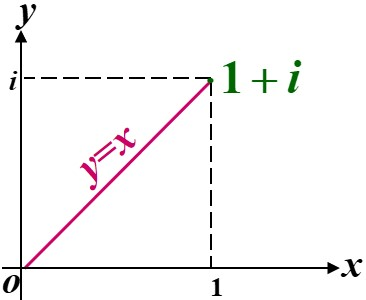
\includegraphics[width=\linewidth]{Figure_3_1_4.jpg}
				\end{figure}
			\end{minipage}
		\end{enumerate}
	\end{solution}
\end{frame}


\begin{frame}
	\begin{solution}
		\begin{enumerate}
			\setcounter{enumi}{1}
			\item The parametric equation of the integration path is $z(t)=t+it^2\ (0\leq t\leq 1)$, so that $\operatorname{Re}z=t$ and $\dif z=(1+2ti)\dif t$, then
			\begin{minipage}[b]{0.55\linewidth}
				$\begin{aligned}
					\int_C \operatorname{Re}z\dif z & =\int_0^1 t(1+2ti)t\dif t                                    \\
					& =\left.\left(\frac{t^2}{2}+\frac{2i}{3}t^3\right)\right|_0^1 \\
					& =\frac{1}{2}+\frac{2}{3}i.
				\end{aligned}$
			\end{minipage}
			\begin{minipage}{0.4\linewidth}
				\begin{figure}
					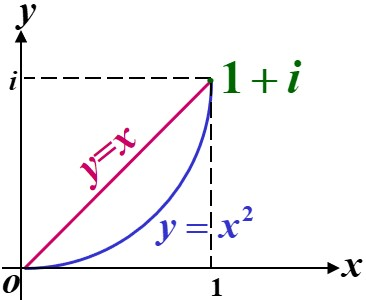
\includegraphics[width=\linewidth]{Figure_3_1_5.jpg}
				\end{figure}
			\end{minipage}
		\end{enumerate}
	\end{solution}
\end{frame}

\begin{frame}
	\begin{solution}
		\begin{enumerate}
			\setcounter{enumi}{2}
			\item The parametric equation of the integration path consists of two straight segments.\\
			The parametric equation of the straight segments on the $x$-axis is $z(t)=t\ (0\leq t\leq 1)$, so that $\operatorname{Re}z=t$ and $\dif z=\dif t$.\\
			The parametric equation of straight segments from $1$ to $1+i$ is $z(t)=1+it\ (0\leq t\leq 1)$, so that $\operatorname{Re}z=1$ and $\dif z=i\dif t$.
			\begin{minipage}[b]{0.55\linewidth}
				$\begin{aligned}
					\int_C \operatorname{Re}z\dif z & =\int_0^1 t\dif t+\int_0^1 1\cdot i\dif t \\
					& =\frac{1}{2}+i.
				\end{aligned}$
			\end{minipage}
			\begin{minipage}{0.4\linewidth}
				\begin{figure}
					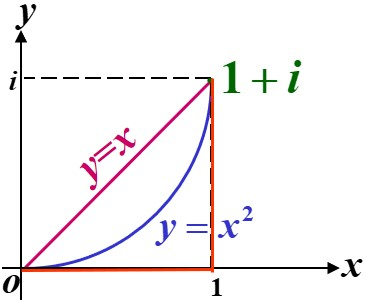
\includegraphics[width=\linewidth]{Figure_3_1_6.jpg}
				\end{figure}
			\end{minipage}
		\end{enumerate}
	\end{solution}
\end{frame}

\begin{frame}
	\begin{example}
		Compute the integral $\int_C |z|\dif z$, where $C$ is the circle $|z|=2$.
	\end{example}
	\begin{solution}<2->
		The parametric equation of the integration path is $z=2e^{i\theta}\ (0\leq\theta\leq 2\pi)$, so that $\dif z=2ie^{i\theta}\dif\theta$, then\\
		$\begin{aligned}
			\int_C |z|\dif z & =\int_0^{2\pi} 2\cdot 2ie^{i\theta}\dif\theta\quad(\text{because of }|z|=2) \\
			& =4i\int_0^{2\pi} (\cos\theta+i\sin\theta)\dif\theta                         \\
			& =0.
		\end{aligned}$
	\end{solution}
\end{frame}

\begin{frame}
	\begin{example}
		Compute the integral $\oint_C \frac{1}{(z-z_0)^{n+1}}\dif z$, where $n$ is an integer, and $C$ is the counterclockwise circle with center $z_0$ and radius $r$.
	\end{example}
	\begin{solution}<2->
		The parametric equation of the integration path is $z=z_0+re^{i\theta}\ (0\leq\theta\leq 2\pi)$,\\
		\begin{minipage}[b]{0.65\linewidth}
			$\begin{aligned}
				\oint_C \frac{1}{(z-z_0)^{n+1}}\dif z & =\int_0^{2\pi} \frac{ire^{i\theta}}{r^{n+1}e^{i(n+1)\theta}}\dif\theta \\
				& =\frac{i}{r^n}\int_0^{2\pi} e^{-in\theta}\dif\theta,
			\end{aligned}$
		\end{minipage}
		\begin{minipage}{0.33\linewidth}
			\begin{figure}
				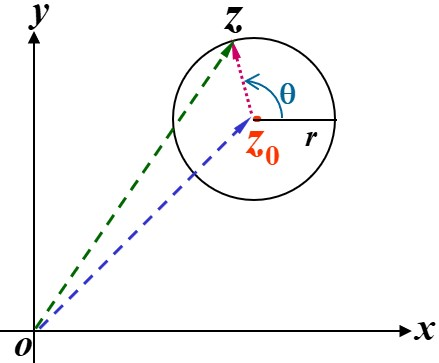
\includegraphics[width=\linewidth]{Figure_3_1_7.jpg}
			\end{figure}
		\end{minipage}
	\end{solution}
\end{frame}

\begin{frame}
	\begin{solution}[Solution\ (Cont.)]
		\begin{minipage}[c]{0.65\linewidth}
			When $n=0$,\\
			$\oint_C \frac{1}{(z-z_0)^{n+1}}\dif z=i\int_0^{2\pi}\dif\theta=2\pi i$.\\
		\end{minipage}
		\begin{minipage}{0.33\linewidth}
			\begin{figure}
				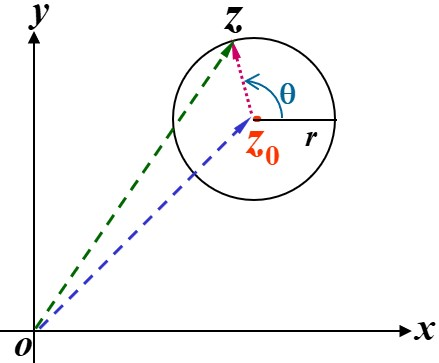
\includegraphics[width=\linewidth]{Figure_3_1_7.jpg}
			\end{figure}
		\end{minipage}\\
		When $n\neq 0$,\\
		$\oint_C \frac{1}{(z-z_0)^{n+1}}\dif z=\frac{i}{r^n}\int_0^{2\pi}(\cos n\theta-i\sin n\theta)\dif\theta=0$.\\
		So $\color{red}\boxed{\color{black}\oint_{|z-z_0|=r}\frac{1}{(z-z_0)^{n+1}}\dif z=\begin{cases}
				2\pi i, & n=0,     \\
				0,      & n\neq 0.
		\end{cases}}$
	\end{solution}
	{\color{blue}Important Conclusion}: The value of the integral is independent of the center and radius of the circle.
\end{frame}



\begin{frame}
	\begin{enumerate}
		\setcounter{enumi}{2}
		\item \textbf{Properties of Complex Integrals}\\
		Complex integrals have similar properties to line integrals of real functions:
		\begin{enumerate}[1)]
			\item $\int_C f(z)\dif z=-\int_{C^-}f(z)\dif z$;
			\item $\int_C kf(z)\dif z=k\int_C f(z)\dif z$; ($k$ is is a constant)
			\item $\int_C \big[f(z)\pm g(z)\big]\dif z=\int_C f(z)\dif z\pm\int_C g(z)\dif z$;
			\item Let the length of curve $C$ be $L$ and function $f(z)$ satisfy $|f(z)|\leq M$ on $C$, then
			\[\left|\int_C f(z)\dif z\right|\leq\int_C |f(z)|\dif s\leq ML. \tag*{Integral estimation inequality}\]
		\end{enumerate}
	\end{enumerate}
\end{frame}

\begin{frame}
	\begin{example}
		Let $C$ be the line segment joining the point $i$ to the point $2+i$ and prove that \[\left|\int_C \frac{1}{z^2}\dif z\right|\leq 2.\]
	\end{example}
	\begin{solution}<2->
		The parametric equation of the line segment $C$ is\\
		$z=(1-t)i+t(2+i)=2t+i\ (0\leq t\leq 1)$,\\
		so that $\left| {{1 \over {{z^2}}}} \right| = {1 \over {|{z^2}|}} = {1 \over {|4{t^2} - 1 + 4ti|}} = {1 \over {4{t^2} + 1}} \le 1$,\\
		then $\left|\int_C \frac{1}{z^2}\dif z\right|\leq 1\times 2=2$.
	\end{solution}
\end{frame}



\begin{frame}
  \begin{enumerate}
    \setcounter{enumi}{3}
    \item \textbf{Summary and Thinking}\\
          In this part, we have learned the definition, existence conditions, calculation and properties of complex integrations. {\color{blue}We should pay attention to that the integration of complex  function has completely similar properties to the line integration in calculus.} In this lesson, we focus on mastering the general computation methods of complex integrals.
  \end{enumerate}
\end{frame}



\begin{frame}
	\begin{example}
		Is the integral definition $\int_C f(z)\dif z$ of complex function $f(z)$ consistent with the definite integral of univariate function?
	\end{example}
\end{frame}



\begin{frame}
	\begin{solution}
		If $C$ is interval $[\alpha,\beta]$ on the real axis, then $\int_C f(z)\dif z=\int_\alpha^\beta f(x)\dif x$. If $f(x)$ is a real valued function, it is the definite integral of a univariate real function. Generally, the integral of function $f(z)$ with starting point $\alpha$ and ending point $\beta$ cannot be written as $\int_\alpha^\beta f(z)\dif z$, because it is a line integral, which must be written as $\int_C f(z)\dif z$,since it is a line integral and must be constrained by the integration path.
	\end{solution}
\end{frame}

\section{Cauchy's Theorem for Simply Connected Domains}

\begin{frame}
  \frametitle{Outline}
  \tableofcontents[currentsection]
\end{frame}




\begin{frame}
	\begin{enumerate}
		\item \textbf{Motivation}
		\begin{enumerate}[i)]
			\item Observe [Example 1.1].\\
			If integrand $f(z)=z$ is analytic everywhere on the entire complex plane, the value of the integral is independent of the path. And we can conclude that the integral of $f(z)=z$ along a closed curve is zero.
			\item Observe [Example 1.4].\\
			When $n=0$, integrand $f(z)=\frac{1}{z-z_0}$ is not analytic everywhere inside the circle $C$ centered on $z_0$, and $\oint_C \frac{1}{z-z_0}\dif z=2\pi i\neq 0$. Although $f(z)$ is analytic everywhere in $C$ except at $z_0$, this domain is no longer a singly connected domain.
		\end{enumerate}
	\end{enumerate}
\end{frame}

\begin{frame}
	\begin{enumerate}
		\item []
		\begin{enumerate}[i)]
			\setcounter{enumii}{2}
			\item Observe [Example 1.5].\\
			Because integrand $f(z)=\overline{z}=x-iy$ does not satisfy the Cauchy-Riemann equations, it is not analytic everywhere in the complex plane.\\
			At this time, the value of the integral $\int_C \overline{z}\dif z$ depends on the path.
		\end{enumerate}
		{\color{blue}From the above discussion, it can be seen that whether the value of the integral is related to the path may depend on the analyticity of the integrand function and the connectivity of the domain.}
	\end{enumerate}
\end{frame}





\begin{frame}
	\begin{enumerate}
		\setcounter{enumi}{1}
		\item \textbf{Cauchy's Theorem for Simply Connected Domains (Cauchy-Goursat Theorem)}
	\end{enumerate}
	\begin{theorem}
		If a function $f$ is analytic in a simply connected domain $B$, then
		\[\int_C f(z)\dif z=0\]
		for every closed curve $C$ lying in $B$.
	\end{theorem}
	\begin{minipage}[b]{0.5\linewidth}
		$C$ in the theorem may not be a simple curve.
	\end{minipage}
	\begin{minipage}{0.45\linewidth}
		\begin{figure}
			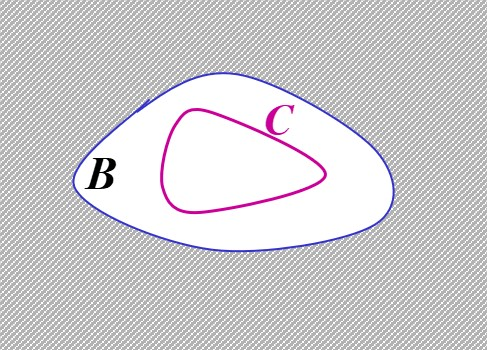
\includegraphics[width=\linewidth]{Figure_3_2_1.jpg}
		\end{figure}
	\end{minipage}
\end{frame}



\begin{frame}
	\begin{enumerate}
		\item []
		Discussions about the theorem:
		\begin{enumerate}[i)]
			\item If the curve $C$ is the boundary of domain $B$, the function $f(z)$ is analytic in $B$ and on $C$, that is, on the closed domain $B=B+C$, then
			\[\oint_C f(z)\dif z.\]
			\item If curve $C$ is the boundary of domain $B$, function $f(x)$ is analytic in $B$ and continuous in the closed domain $B=B+C$, then the theorem is still valid.
		\end{enumerate}
	\end{enumerate}
\end{frame}




\begin{frame}
  \begin{enumerate}
    \item []
          \begin{figure}
            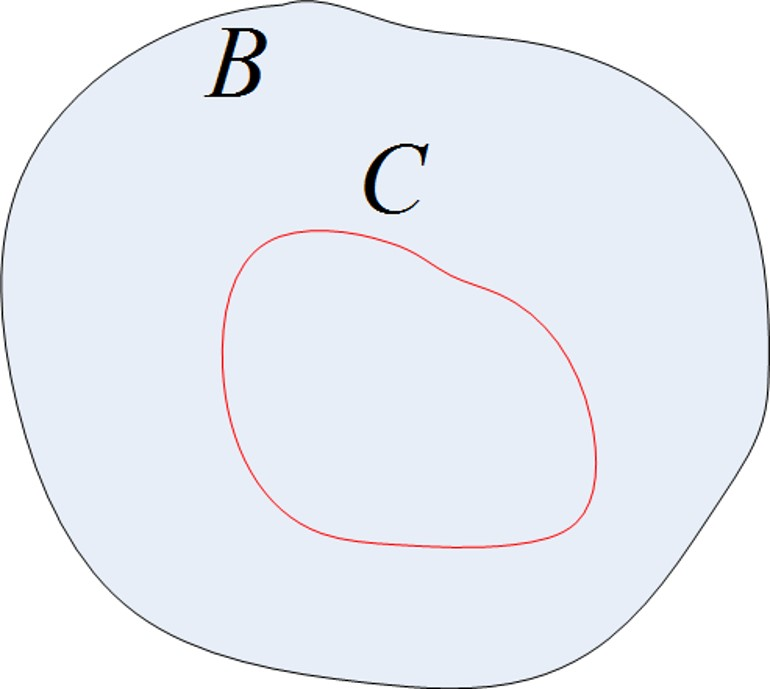
\includegraphics[height=0.7\textheight]{Figure_3_2_2.jpg}
          \end{figure}
  \end{enumerate}
\end{frame}

\begin{frame}
  \begin{enumerate}
    \item []
          \begin{figure}
            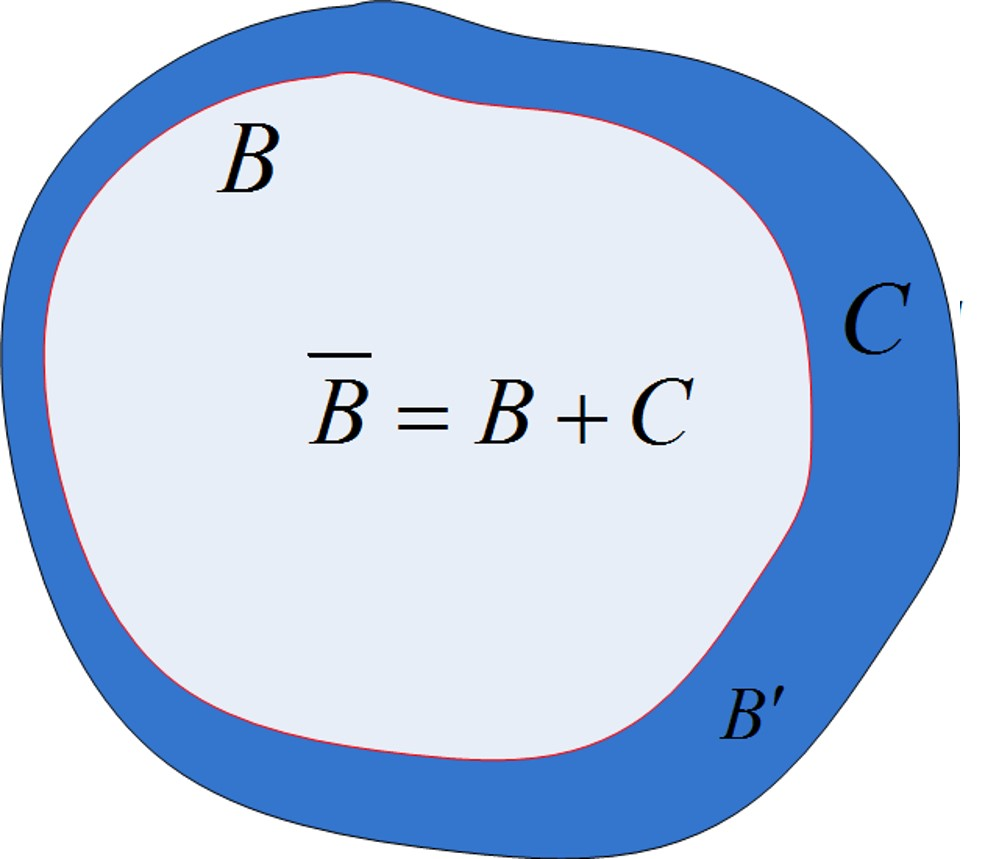
\includegraphics[height=0.7\textheight]{Figure_3_2_3.jpg}
          \end{figure}
  \end{enumerate}
\end{frame}

\begin{frame}
  \begin{enumerate}
    \item []
          \begin{figure}
            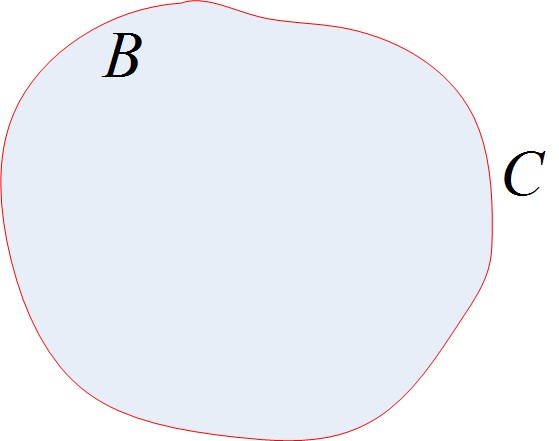
\includegraphics[height=0.7\textheight]{Figure_3_2_4.jpg}
          \end{figure}
  \end{enumerate}
\end{frame}




\begin{frame}
	\begin{enumerate}
		\setcounter{enumi}{2}
		\item \textbf{Examples}
	\end{enumerate}
	\begin{example}
		Compute the integral $\oint_{|z|=1} \frac{1}{2z-3}\dif z$.
	\end{example}
	\begin{solution}<2->
		Since $f(z)$ is analytic in $|z|\leq 1$, according to Cauchy's Theorem, we have \\ $\oint_{|z|=1} \frac{1}{2z-3}\dif z=0$.
	\end{solution}
\end{frame}



\begin{frame}
	\begin{example}
		Compute the integral $\oint_{|z-i|=\frac{1}{2}} \frac{1}{z(z^2+1)}\dif z$.
	\end{example}
	\begin{solution}<2->
		$\frac{1}{z(z^2+1)}=\frac{1}{z}-\frac{1}{2}\left(\frac{1}{z+i}+\frac{1}{z-i}\right)$.\\
		Because $\frac{1}{z}$ and $\frac{1}{z+i}$ are analytic in $|z-i|\leq\frac{1}{2}$,\\
		according to Cauchy's Theorem,
	\end{solution}
\end{frame}

\begin{frame}
	\begin{solution}
		\begin{align*}
			& \oint_{|z-i|=\frac{1}{2}} \frac{1}{z(z^2+1)}\dif z                                                         \\
			= & \oint_{|z-i|=\frac{1}{2}} \left(\frac{1}{z}-\frac{1}{2}\frac{1}{z+i}-\frac{1}{2}\frac{1}{z-i}\right)\dif z \\
			= & \begin{aligned}[t]
				\color{red}\boxed{\color{black}\oint_{|z-i|=\frac{1}{2}} \frac{1}{z}\dif z-\frac{1}{2}\oint_{|z-i|=\frac{1}{2}} \frac{1}{z+i}\dif z} \\
				\color{red}=0                                                                                                                        \\
			\end{aligned}-\frac{1}{2}\oint_{|z-i|=\frac{1}{2}} \frac{1}{z-i}\dif z                        \\
			= & -\frac{1}{2}\oint_{|z-i|=\frac{1}{2}} \frac{1}{z-i}\dif z=-\frac{1}{2}\cdot 2\pi i=-\pi i.
		\end{align*}
	\end{solution}
\end{frame}

\begin{frame}
	\begin{enumerate}
		\setcounter{enumi}{3}
		\item \textbf{Summary and Thinking}\\
		In this part, we focus on mastering Cauchy's Theorem for simply connected domains:\\
		{\color{blue}
			If a function $f$ is analytic throughout a simply connected domain $B$, then
			\[\int_C f(z)\dif z=0\]
			for every closed curve $C$ lying in $B$.}\\
		Pay attention to the conditions under which the theorem holds.
	\end{enumerate}
\end{frame}

\begin{frame}
	\begin{example}
		What should we pay attention to in the application of Cauchy's Theorem?
	\end{example}
\end{frame}

\begin{frame}
	\begin{solution}
		\begin{enumerate}[i)]
			\item Note the condition "simply connected domain" in the theorem.\\
			Counter example: $f(z)=\frac{1}{z}$ in the ring  $\frac{1}{2}\leq |z|\leq\frac{3}{2}$.
			\item Note that the theorem cannot be used in reverse.\\
			{\color{red}We cannot get $f(z)$ is analytic in the domain enclosed by $C$ from $\oint_C f(z)\dif z=0$.}\\
			Counter example: $f(z)=\frac{1}{z^2}$ in $|z|=1$.
		\end{enumerate}
	\end{solution}
\end{frame}






\section{Cauchy's Theorem for Multiply Connected Domains}

\begin{frame}
  \frametitle{Outline}
  \tableofcontents[currentsection]
\end{frame}

\begin{frame}
	\begin{enumerate}
		\item \textbf{Motivation}\\
		For example, compute the integral $\oint_{|z-1|=2}\frac{1}{z-1}\dif z$.\\
		We see that $|z|=2$ is the closed curve surrounding point $z=1$.\\
		And, according to [Example 1.4], we have $\oint_{|z-1|=2}\frac{1}{z-1}\dif z=2\pi i$.\\
		We hope that the theorem can be extended to multiply connected domains.
	\end{enumerate}
\end{frame}



\begin{frame}
	\begin{enumerate}
		\setcounter{enumi}{1}
		\item \textbf{Cauchy's Theorem for Multiply Connected Domains}
		\begin{enumerate}[1)]
			\item Principle of Deformation of Paths\\
			Let the function $f(z)$ be analytic in a multiply connected domain $D$, $C$ and $C_1$ are any two simple closed curves in the multiply connected domain $D$ (Their positive directions of $C$ and $C_1$ are counterclockwise).\\
			Moreover, we assume that $C_1$ is in $C$ and $D_1$ bounded by $C$ and $C_1$ is all contained in $D$.\\
			Make two disjoint arc segments $\wideparen{AA'}$ and $\wideparen{BB'}$.
			\begin{figure}
				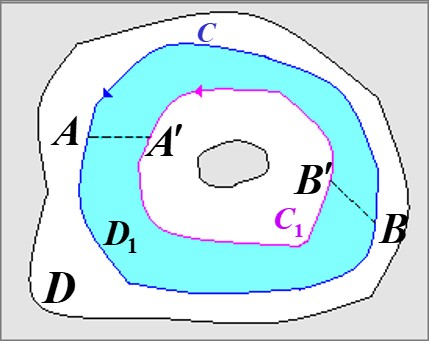
\includegraphics[width=0.5\linewidth]{Figure_3_3_1.jpg}
			\end{figure}
		\end{enumerate}
	\end{enumerate}
\end{frame}

\begin{frame}
	
	\begin{enumerate}
		\item []
		For the convenience of discussion, the points $E$, $E'$, $F$ and $F'$ are added as shown in the figure. Obviously, the curves $AEBB'E'A'A$ and $AA'F'B'BFA$ are closed curves.\\
		Because they are all contained in $D$, we must have according to Cauchy's Theorem for simply connected domains: \\                  
		$\oint_{AEBB'E'A'A}f(z)\dif z=0$, $\oint_{AA'F'B'BFA}f(z)\dif z=0$. \\
		$AEBB'E'A'A=AEB+BB'+B'E'A'+A'A$,\\
		$AA'F'B'BFA=AA'+A'F'B'+B'B+BFA$.           
		\begin{figure}
			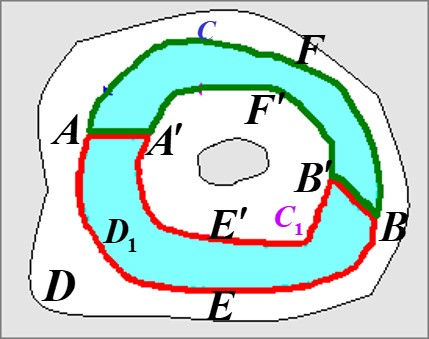
\includegraphics[width=0.4\linewidth]{Figure_3_3_2.jpg}
		\end{figure}    
	\end{enumerate}
\end{frame}

\begin{frame}
	
	\begin{enumerate}
		\item []
		From $\oint_{AEBB'E'A'A}f(z)\dif z+\oint_{AA'F'B'BFA}f(z)\dif z=0$, we have: \\
		$\begin{aligned}
			\oint_{C}f(z)\dif z+\oint_{C_1^-}f(z)\dif z+\oint_{\wideparen{AA'}}f(z)\dif z+\oint_{\wideparen{A'A}}f(z)\dif z \\
			+\oint_{\wideparen{B'B}}f(z)\dif z+\oint_{\wideparen{BB'}}f(z)\dif z=0
		\end{aligned}$\\
		
		That is
		$\oint_{C}f(z)\dif z+\oint_{C_1^-}f(z)\dif z=0$,\\
		or $\oint_{C}f(z)\dif z=\oint_{C_1}f(z)\dif z$.
		\begin{figure}
			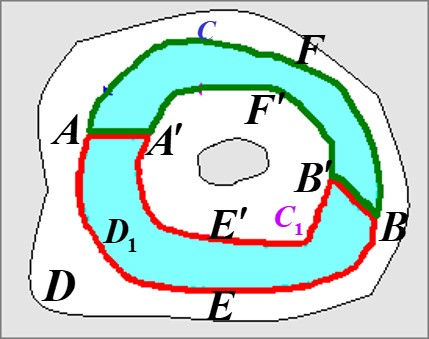
\includegraphics[width=0.4\linewidth]{Figure_3_3_2.jpg}
		\end{figure}
	\end{enumerate}
	
\end{frame}


\begin{frame}
	
	\begin{enumerate}
		\item []
		
		$\begin{aligned}[t]
			\oint_{\Gamma}f(z)\dif z=0 & \Rightarrow\oint_{C}f(z)\dif z+\oint_{C_1^-}f(z)\dif z=0 \\
			& \Rightarrow\oint_{C}f(z)\dif z=\oint_{C_1}f(z)\dif z
		\end{aligned}$\\
		{\color{blue}Principle of deformation of paths}: The integral of an analytic function along a closed curve in the domain does not change its value due to the continuous deformation of the closed curve in the domain, as long as the curve does not pass through the point where the function $f(z)$ cannot be analytic in the deformation process.
		
		
		\begin{figure}
			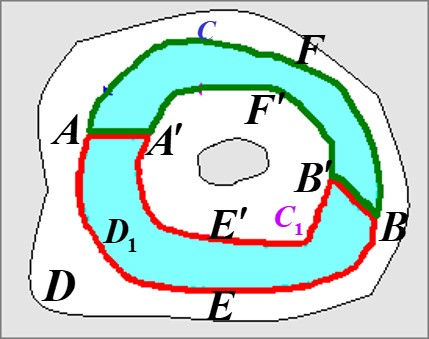
\includegraphics[width=0.4\linewidth]{Figure_3_3_2.jpg}
		\end{figure}
		
	\end{enumerate}
	
\end{frame}



\begin{frame}
	\setcounter{enumi}{2}
	\begin{enumerate}[2)]

		\item Cauchy's Theorem for Multiply Connected Domains
	\end{enumerate}
	
	\begin{theorem}
		Let $C$ be a simple closed curve in the multiply connected domain $D$, and $C_1$, $C_2$, $\cdots$, $C_n$ are simple closed curves in $C$, which do not contain or intersect each other, and the domains bounded by $C_1$, $C_2$, $\cdots$, $C_n$ are all contained in $D$. If $f(x)$ is analytic in $D$, then
		\begin{enumerate}
			\item \begin{minipage}[t]{0.5\linewidth}
				$\oint_{C}f(z)\dif z=\sum_{k=1}^{n}\oint_{C_k}f(z)\dif z$,\\
				where the positive directions of $C$ and $C_k$ are counterclockwise.
			\end{minipage}
			\ \
			\begin{minipage}[t]{0.4\linewidth}
				\begin{figure}
					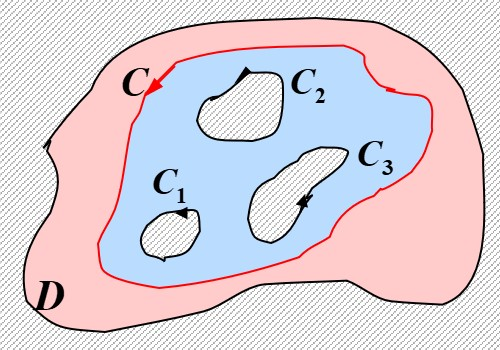
\includegraphics[width=\linewidth]{Figure_3_3_3.jpg}
				\end{figure}
			\end{minipage}
		\end{enumerate}
	\end{theorem}
\end{frame}




\begin{frame}
	\setcounter{theorem}{0}
	\begin{theorem}[Cont.]
		\begin{enumerate}
			\setcounter{enumi}{1}
			\item \begin{minipage}[t]{0.5\linewidth}
				$\oint_{\Gamma}f(z)\dif z=0$, where $\Gamma$ is a composite closed curve composed of $C$ and $C_k (k=1,2,\cdots,n)$, and the positive direction of $C$ is counterclockwise, the positive direction of $C_k$ is clockwise, i.e., $\Gamma=\{C,C_1^-,C_2^-, ..., C_n^- \}$.
			\end{minipage}
			\ \
			\begin{minipage}[t]{0.4\linewidth}
				\begin{figure}
					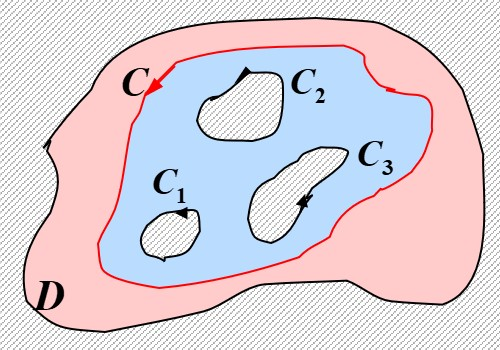
\includegraphics[width=\linewidth]{Figure_3_3_3.jpg}
				\end{figure}
			\end{minipage}
		\end{enumerate}
	\end{theorem}
\end{frame}








\begin{frame}
	\begin{enumerate}
		\setcounter{enumi}{2}
		\item \textbf{Examples}
	\end{enumerate}
	\begin{example}
		Compute the integral $\oint_{\Gamma}\frac{2z-1}{z^2-z}\dif z$, where $\Gamma$ is any positive simple closed curve surrounding circle $|z|=1$.
	\end{example}
	\begin{solution}<2->
		\begin{minipage}[b]{0.5\linewidth}
			$\frac{2z-1}{z^2-z}$ has two singularities $z=0$ and $z=1$ in the complex plane. $\Gamma$ contains both singularities.
		\end{minipage}
		$\quad$
		\begin{minipage}{0.4\linewidth}
			\begin{figure}
				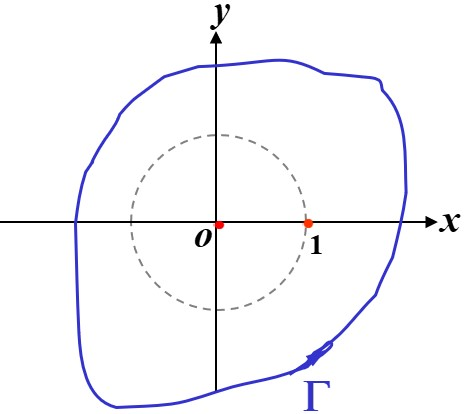
\includegraphics[width=\linewidth]{Figure_3_3_4.jpg}
			\end{figure}
		\end{minipage}
	\end{solution}
\end{frame}

\begin{frame}
	\begin{solution}[Solution\ (Cont.)]
		We make two positive circles $C_1$ and $C_2$ in $\Gamma$ that do not contain or intersect each other, and $C_1$ contains only singularity $z=0$, $C_2$ contains only singularity $z=1$.\\
		According Cauchy's Theorem for multiply connected domains,\\
		\begin{minipage}[b]{0.5\linewidth}
			$\begin{aligned}
				& \oint_{\Gamma}\frac{2z-1}{z^2-z}\dif z                                  \\
				= & \oint_{C_1}\frac{2z-1}{z^2-z}\dif z+\oint_{C_2}\frac{2z-1}{z^2-z}\dif z \\
				= & \oint_{C_1}\frac{1}{z-1}\dif z+\oint_{C_1}\frac{1}{z}\dif z             \\
				& +\oint_{C_2}\frac{1}{z-1}\dif z+\oint_{C_2}\frac{1}{z}\dif z            \\
				= & 0+2\pi i+2\pi i+0=4\pi i.
			\end{aligned}$
		\end{minipage}
		$\quad$
		\begin{minipage}{0.4\linewidth}
			\begin{figure}
				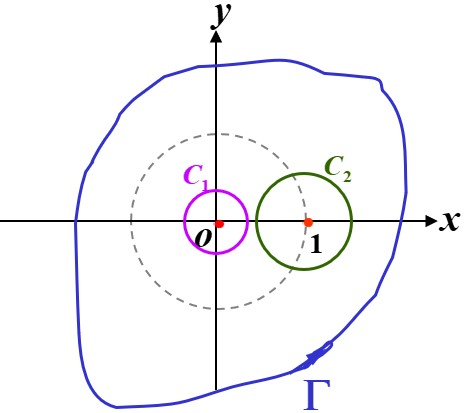
\includegraphics[width=\linewidth]{Figure_3_3_5.jpg}
			\end{figure}
		\end{minipage}
	\end{solution}
\end{frame}

\begin{frame}
	\begin{example}
		Compute the integral $\oint_{\Gamma}\frac{e^z}{z}\dif z$, where $\Gamma$ is composed of positive circle $|z|=2$ and negative circle $|z|=1$.
	\end{example}
	\begin{solution}<2->
		\begin{minipage}[c]{0.5\linewidth}
			$C_1$ and $C_2$ form a ring domain, $\frac{e^z}{z}$ is analytic in the ring domain and its boundary, the boundary of the ring domain forms a composite closed curve. \\
			According Cauchy's Theorem for multiply connected domains, $\oint_{\Gamma}\frac{e^z}{z}\dif z=0$.
		\end{minipage}
		$\quad$
		\begin{minipage}[T]{0.4\linewidth}
			\begin{figure}
				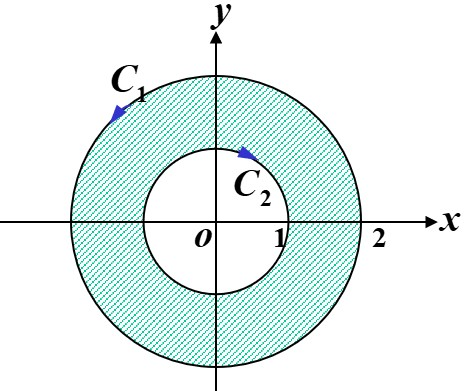
\includegraphics[width=\linewidth]{Figure_3_3_6.jpg}
			\end{figure}
		\end{minipage}
	\end{solution}
\end{frame}

\begin{frame}
	\begin{example}
		Compute the integral $\oint_{\Gamma}\frac{1}{(z-a)^{n+1}}\dif z$, where $\Gamma$ is any simple closed curve that encircles $a$, and $n$ is an integer.
	\end{example}
	\begin{solution}<2->
		\begin{minipage}[c]{0.5\linewidth}
			Because $a$ is inside the closed curve $\Gamma$, a small positive number $\rho$ can be taken to make circle $\Gamma_1:|z-a|=\rho$ inside $\Gamma$.\\
			$f(z)=\frac{1}{(z-a)^{n+1}}$ is analytic in a multiply connected domain bounded by $\Gamma+\Gamma_1^-$.
		\end{minipage}
		$\quad$
		\begin{minipage}[T]{0.4\linewidth}
			\begin{figure}
				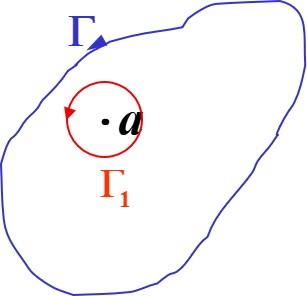
\includegraphics[width=\linewidth]{Figure_3_3_7.jpg}
			\end{figure}
		\end{minipage}
	\end{solution}
\end{frame}

\begin{frame}
	\begin{solution}
		According to Cauchy's Theorem for multiply connected domains,\\
		\begin{minipage}[c]{0.6\linewidth}
			$\oint_{\Gamma}\frac{1}{(z-a)^{n+1}}\dif z=\oint_{\Gamma_1}\frac{1}{(z-a)^{n+1}}\dif z$.\\
			Let $z=a+\rho e^{i\theta}\ 0<\theta\leq 2\pi$,\\
			$\begin{aligned}
				\oint_{\Gamma}\frac{1}{(z-a)^{n+1}}\dif z & =\int_{0}^{2\pi}\frac{\rho ie^{i\theta}}{(\rho e^{i\theta})^{n+1}}\dif\theta \\
				& =\int_{0}^{2\pi}\frac{ie^{-in\theta}}{\rho^n}\dif\theta
			\end{aligned}$
			So {\color{blue}$\boxed{\color{black}\oint_{\Gamma}\frac{1}{(z-a)^{n+1}}\dif z=\begin{cases}
						2\pi i, & n=0     \\
						0,      & n\neq 0
				\end{cases}}$}.
		\end{minipage}
		\begin{minipage}[T]{0.35\linewidth}
			\begin{figure}
				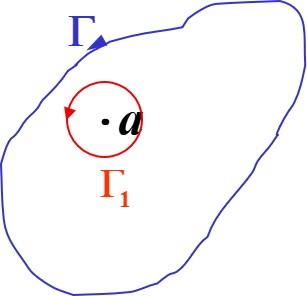
\includegraphics[width=\linewidth]{Figure_3_3_7.jpg}
			\end{figure}
		\end{minipage}
	\end{solution}
	{\color{blue}This conclusion is very important and convenient to use, because $\Gamma$ does not have to be a circle, and $a$ does not have to be the center of a circle, as long as $a$ is in a simple closed curve $\Gamma$.}
\end{frame}

\begin{frame}
	\begin{example}
		Compute the integral $\frac{1}{2\pi i}\oint_{\Gamma}\frac{1}{(z-z_0)^n}\dif z$, where $\Gamma$ is any positive closed curve encircling $z_0$, and $n$ is a natural number.
	\end{example}
	\begin{solution}<2->
		As can be seen from the above example,\\
		$\oint_{\Gamma}\frac{1}{(z-a)^{n+1}}\dif z=\begin{cases}
			2\pi i, & n=0      \\
			0,      & n\neq 0.
		\end{cases}$\\
		Let $a=z_0$,\\
		then $\frac{1}{2\pi i}\oint_{\Gamma}\frac{1}{(z-z_0)^n}\dif z=\begin{cases}
			1, & n=1      \\
			0, & n\neq 1.
		\end{cases}$
	\end{solution}
\end{frame}


\begin{frame}
	\begin{example}
		Prove $\oint_C (z-\alpha)^n\dif z=0\ (n\neq-1)$, where $C$ is an arbitrary closed curve.
	\end{example}
	\begin{solution}<2->
		
		\begin{enumerate}
			\item If $\alpha$ is not in $C$, $(z-\alpha)^n$ is analytic on $C$ and inside $C$. Thus, we have $\oint_C (z-\alpha)^n\dif z=0\ $.
			
			\item If $\alpha$ is in $C$, since we have\\
			$\oint_{\Gamma}\frac{1}{(z-\alpha)^{n'+1}}\dif z=\begin{cases}
				2\pi i, & n'=0      \\
				0,      & n'\neq 0.
			\end{cases}$ \\		
			and $n\neq -1$, we have $\oint_C (z-\alpha)^n\dif z=0\ $
		\end{enumerate}
	\end{solution}
\end{frame}



\begin{frame}
	\begin{enumerate}
		\setcounter{enumi}{3}
		\item \textbf{Summary and Thinking}\\
		Cauchy's Theorem is important in complex integration. Mastering and flexibly applying it is the difficulty of this chapter.\\
		Common conclusions:
		\[\oint_{\Gamma}\frac{1}{(z-a)^{n+1}}\dif z=\begin{cases}
			2\pi i, & n=0      \\
			0,      & n\neq 0.
		\end{cases}\]
	\end{enumerate}
\end{frame}

\begin{frame}
	\begin{example}
		What is the use of Cauchy's Theorem for multiply connected domains in integral calculation? What should we pay attention to?
	\end{example}
\end{frame}

\begin{frame}
	\begin{solution}
		Using Cauchy's Theorem for multiply connected domains is the main method to calculate the integral along the closed curve.\\
		When using Cauchy's Theorem for multiply connected domains, pay attention to the direction of the curve.
	\end{solution}
\end{frame}

\section{Antiderivative}

\begin{frame}
  \frametitle{Outline}
  \tableofcontents[currentsection]
\end{frame}

\begin{frame}
  \begin{enumerate}
    \item \textbf{Main Theorems and Definitions}\\
          \begin{enumerate}[1)]          	
          	           \item Two Main Theorems
          \end{enumerate}
  \end{enumerate}
  \begin{theorem}
    If $f(z)$ is analytic everywhere in simply connected domain $B$, then the integral $\int_C f(z)\dif z$ is independent of the path $C$ connecting the starting point and the ending point.
  \end{theorem}
  From this theorem, it can be seen that the integral of an analytical function in a simply connected domain is only related to the starting point $z_0$ and the ending point $z_1$ (see the figure on the next slice).
\end{frame}

\begin{frame}

          \begin{enumerate}
            \item []
                  \begin{figure}
                    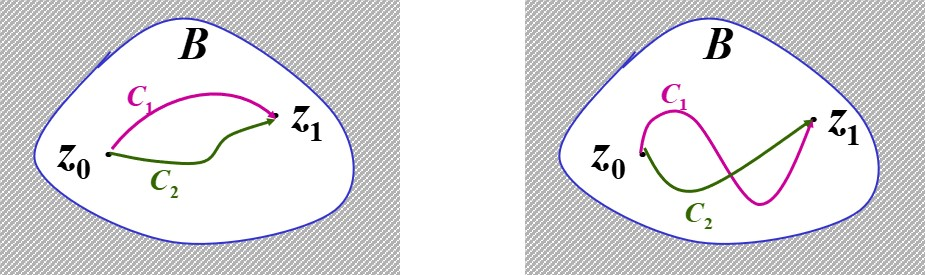
\includegraphics[width=\linewidth]{Figure_3_4_1.jpg}
                  \end{figure}
                  \[\int_{C_1}f(z)\dif z=\int_{C_2}f(z)\dif z=\int_{z_0}^{z_1}f(z)\dif z\]
                  If $z_0$ is fixed, let $z_1$ change within $B$ and make $z_1=z$, then we can determine a single-valued function in $B$ as the following: $$F(z)=\int_{z_0}^{z}f(\zeta)\dif\zeta$$ 
          \end{enumerate}

\end{frame}

\begin{frame}
  \begin{theorem}
    If $f(z)$ is analytic everywhere in simply connected domain $B$, then the integral  $F(z)=\int_{z_0}^{z}f(\zeta)\dif\zeta$ must be an analytical function in $B$; and we have $F'(z)=f(z)$
  \end{theorem}
  \begin{proofs}<2->
    \begin{minipage}[b]{0.65\linewidth}
      Prove this theorem using the definition of derivative.\\
      Let $z$ be an any point in $B$ and make a small circle $K$ contained in $B$ centered on $z$.
    \end{minipage}
    \begin{minipage}{0.3\linewidth}
      \begin{figure}
        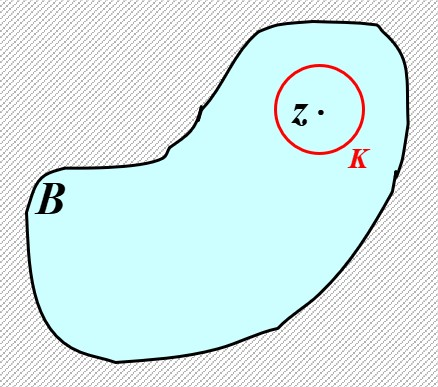
\includegraphics[width=\linewidth]{Figure_3_4_2.jpg}
      \end{figure}
    \end{minipage}
  \end{proofs}
\end{frame}

\begin{frame}
  \begin{proofs}[\proofname\ (Cont.)]
    Let $|\Delta z|$ be sufficiently small so that $z+\Delta z$ is always within the small circle $K$. As defined by $F(z)$, $F(z+\Delta z)-F(z)=\int_{z_0}^{z+\Delta z}f(\zeta)\dif\zeta-\int_{z_0}^{z}f(\zeta)\dif\zeta$.\\
    \begin{minipage}[b]{0.65\linewidth}
      Because the integrals are independent of the paths, the integral path of $\int_{z_0}^{z+\Delta z}f(\zeta)\dif\zeta$ can go from $z_0$ to $z$ along the same path of $\int_{z_0}^{z}f(\zeta)\dif\zeta$, then go along the straight line from $z$ to $z+\Delta z$.
    \end{minipage}
    \begin{minipage}[b]{0.3\linewidth}
      \begin{figure}
        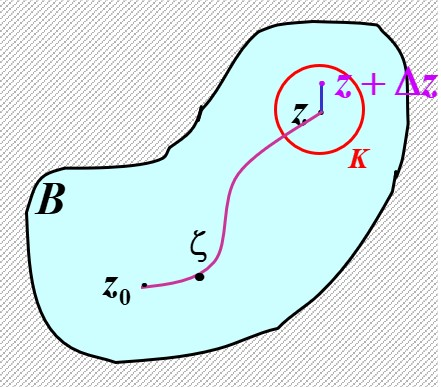
\includegraphics[width=\linewidth]{Figure_3_4_3.jpg}
      \end{figure}
    \end{minipage}
  \end{proofs}
\end{frame}

\begin{frame}
  \begin{proofs}[\proofname\ (Cont.)]
    Then $F(z+\Delta z)-F(z)=\int_{z}^{z+\Delta z}f(\zeta)\dif\zeta$.\\
    Since $\int_{z}^{z+\Delta z}f(z)\dif\zeta=f(z)\int_{z}^{z+\Delta z}\dif\zeta=f(z)\Delta z$, we have \\
    \begin{minipage}[T]{0.55\linewidth}
      $\begin{aligned}
            & \frac{F(z+\Delta z)-F(z)}{\Delta z}-f(z)                                \\
          = & {1 \over {\Delta z}}\left[ {\int_z^{z + \Delta z} {f(\zeta ){\rm{d}}\zeta  - f(z)\Delta z} } \right]     \\
          = & \frac{1}{\Delta z}\int_{z}^{z+\Delta z}\big[f(\zeta)-f(z)\big]\dif\zeta
        \end{aligned}$
    \end{minipage}
    \begin{minipage}{0.4\linewidth}
      \begin{figure}
        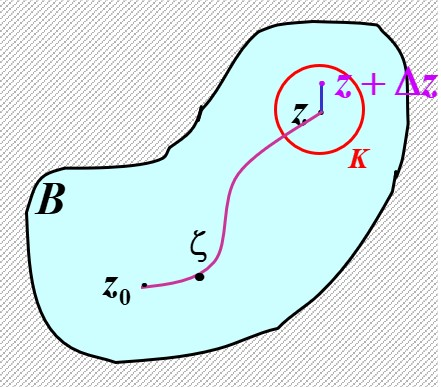
\includegraphics[width=\linewidth]{Figure_3_4_3.jpg}
      \end{figure}
    \end{minipage}
  \end{proofs}
\end{frame}

\begin{frame}
  \begin{proofs}[\proofname\ (Cont.)]
    Because $f(z)$ is analytic in $B$, it gives that $f(z)$ is continuous in $B$.\\
    \begin{minipage}[T]{0.55\linewidth}
      And $\forall\varepsilon>0,\exists\delta>0$, so that for all $\zeta$ satisfying $|\zeta-z|<\delta$ is in $B$, there is always $|f(\zeta)-f(z)|<\varepsilon$.\\
      According to integral estimation inequality, when $|\Delta z|<\delta$, we have m n\\
      $\left|\frac{F(z+\Delta z)-F(z)}{\Delta z}-f(z)\right|$
    \end{minipage}
    \begin{minipage}{0.4\linewidth}
      \begin{figure}
        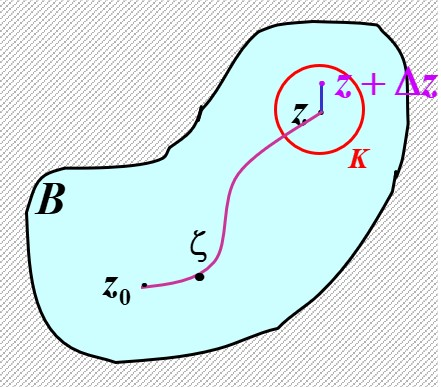
\includegraphics[width=\linewidth]{Figure_3_4_3.jpg}
      \end{figure}
    \end{minipage}
  \end{proofs}
\end{frame}

\begin{frame}
  \begin{proof}[\proofname\ (Cont.)]
    $\begin{aligned}
             & \left|\frac{F(z+\Delta z)-F(z)}{\Delta z}-f(z)\right|                                  \\
        =    & \frac{1}{|\Delta z|}\left|\int_{z}^{z+\Delta z}\big[f(\zeta)-f(z)\big]\dif\zeta\right| \\
        \leq & \frac{1}{|\Delta z|}\int_{z}^{z+\Delta z}\left|f(\zeta)-f(z)\right|\dif S              \\
        \leq & \frac{1}{|\Delta z|}\cdot\varepsilon\cdot|\Delta z|=\varepsilon.
      \end{aligned}$\\
    So $\lim_{\Delta z\to 0}\left|\frac{F(z+\Delta z)-F(z)}{\Delta z}-f(z)\right|=0$,\\
    that is $F'(z)=f(z)$.
  \end{proof}
  {\color{blue}This theorem is completely similar to the fundamental theorem of calculus.}
\end{frame}

\begin{frame}
\begin{enumerate}[2)]
     \item Definition of Antiderivative\\
            \begin{itemize}
            	\item If the derivative of function $\phi(z)$ in domain $B$ is $f(x)$, that is, $\phi'(z)=f(z)$, then $\phi(z)$ is called an antiderivative of $f(x)$ in domain $B$.
            	\item   Obviously, $F(z)=\int_{z_0}^{z}f(\zeta)\dif\zeta$ is an antiderivative of $f(z)$.
            	\item  Relationship between antiderivatives:\\
            	Any two antiderivatives of $f(z)$ differ by a constant.
            	
            \end{itemize}
     
          \end{enumerate}

\end{frame}

\begin{frame}
  \begin{proof}
    Let $G(z)$ and $H(z)$ be any two antiderivatives of $f(z)$,\\
    then $\begin{aligned}[t]
        \big[G(z)-H(z)\big]' & =G'(z)-H'(z)        \\
                             & =f(z)-f(z)\equiv 0,
      \end{aligned}$\\
    that is $G(z)-H(z)=c$ ($c$ is any constant).
  \end{proof}
  It can be seen that if $f(z)$ has an antiderivative $F(z)$ in the domain $B$, it must have infinite number of  antiderivatives $F(z)+c$ ($c$ is any constant).
\end{frame}

\begin{frame}

    \begin{enumerate} [3)]

            \item Definition of Infinite Integral\\
                  The general expression $F(z)+c$ ($c$ is any constant) of the original function of $f(z)$ is called the indefinite integral of $f(z)$, and written as
                  \[\int f(z)\dif z=F(z)+c.\]

  \end{enumerate}
  \begin{theorem}[similar to Newton-Leibniz formula]
    If $f(z)$ is analytic in simply connected domain $B$, $F(z)$ is an antiderivative of $f(z)$, then
    \[\int_{z_0}^{z_1}f(z)\dif z=F(z_1)-F(z_0),\]
    where $z_0$ and $z_1$ are in $B$.
  \end{theorem}
\end{frame}

\begin{frame}
  \begin{proof}
    Because $\int_{z_0}^{z}f(z)\dif z$ is an antiderivative of $f(z)$,\\
    $\int_{z_0}^{z}f(z)\dif z=F(z)+c$.\\
    When $z=z_0$, according to Cauchy's Theorem for simply connected domains, $c=-F(z_0)$,\\
    so $\int_{z_0}^{z}f(z)\dif z=F(z)-F(z_0)$, or $\int_{z_0}^{z_1}f(z)\dif z=F(z_1)-F(z_0)$.
  \end{proof}
  With the above theorem, the integral of a complex function can be calculated in a similar way as in calculus.
\end{frame}

\begin{frame}
  \begin{enumerate}
    \setcounter{enumi}{1}
    \item \textbf{Examples}
  \end{enumerate}
  \begin{example}
    Compute the integral $\int_{z_0}^{z_1}z\dif z$.
  \end{example}
  \begin{solution}<2->
    Function $f(z)=z$ is an analytic function,
    and its antiderivative is $\frac{1}{2}z^2$.\\
    According to Newton-Leibniz formula,\\
    $\int_{z_0}^{z_1}z\dif z=\left.\frac{1}{2}z^2\right|_{z_0}^{z_1}=\frac{1}{2}(z_1^2-z_0^2)$.
  \end{solution}
\end{frame}

\begin{frame}
  \begin{example}
    Compute the integral $\int_{0}^{\pi i}z\cos z^2\dif z$.
  \end{example}
  \begin{solution}<2->
    $\begin{aligned}
        \int_{0}^{\pi i}z\cos z^2\dif z & =\frac{1}{2}\int_{0}^{\pi i}\cos z^2\dif z^2    \\
                                        & =\left.\frac{1}{2}\sin z^2\right|_{0}^{\pi i}   \\
                                        & =\frac{1}{2}\sin(-\pi^2)=-\frac{1}{2}\sin\pi^2.
      \end{aligned}$
  \end{solution}
\end{frame}

\begin{frame}
  \begin{example}
    Compute the integral $\int_{1}^{1+i}ze^z\dif z$.
  \end{example}
  \begin{solution}<2->
    According to integration by parts formula,\\
    $(z-1)e^z$ is an antiderivative of $ze^z$,\\
    $\int_{1}^{1+i}ze^z\dif z=(z-1)e^z\big|_{1}^{1+i}=ie^{1+i}=ie(\cos 1+i\sin 1)$.
  \end{solution}
\end{frame}

\begin{frame}
  \begin{example}
    Compute the integral $\int_{1}^{i}\frac{\ln(z+1)}{z+1}\dif z$, where circle $|z|=1$ lies in domain $\operatorname{Im}(z)\geq 0,\operatorname{Re}(z)\geq 0$.
  \end{example}
  \begin{solution}<2->
    $\frac{\ln(z+1)}{z+1}$ is analytic in its domain,\\
    its antiderivative is $\frac{\ln^2(z+1)}{2}$.\\
    $\begin{aligned}
        \int_{1}^{i}\frac{\ln(z+1)}{z+1}\dif z & =\left.\frac{\ln^2(z+1)}{2}\right|_{1}^{i}=\frac{1}{2}\big[\ln^2 (1+i)-\ln^2 2\big] \\
                                               & =\frac{1}{2}\left[\left(\frac{1}{2}\ln 2+\frac{\pi}{4}i\right)^2-\ln^2 2\right]     \\
                                               & =-\frac{\pi^2}{32}-\frac{3}{8}\ln^2 2+\frac{\pi\ln 2}{8}i.
      \end{aligned}$
  \end{solution}
\end{frame}

\begin{frame}
  \begin{enumerate}
    \setcounter{enumi}{3}
    \item \textbf{Summary and Thinking}\\
          This part introduces the definitions of antiderivative and Newton-Leibniz formula.\\
          We should pay attention to the combination with the relevant contents in calculus to better understand the contents of this part.\\
          \vspace{\baselineskip}
          \color{blue}
          $F(z)=\int_{z_0}^{z}f(\zeta)\dif\zeta\quad\int f(z)\dif z=F(z)+c$\\
          $\int_{z_0}^{z_1}f(z)\dif z=G(z_1)-G(z_0)$
  \end{enumerate}
\end{frame}

\begin{frame}
  \begin{example}
    What are the similarities and differences between the Newton-Leibniz formula for the integration of analytic complex functions in a simply connected domain and the Newton-Leibniz formula for the definite integration of real functions?
  \end{example}
\end{frame}

\begin{frame}
  \begin{solution}
    {\color{red}The formulation and results are similar.}\\
    In complex integration, $f(z)$ is required to be an analytical function in a simply connected domain, and the integration path is curve $C$, so $z_0$ and $z$ are complex numbers;\\
    In real integral, $f(x)$ is required to be a continuous real function over interval $[a,b]$, where $a$ and $x$ are real numbers.\\
    {\color{red}There are great differences in the requirements for functions between them: analytic vs. continuous.}
  \end{solution}
\end{frame}

\section{Cauchy's Integral Formula}

\begin{frame}
  \frametitle{Outline}
  \tableofcontents[currentsection]
\end{frame}

\begin{frame}
  \setlength{\baselineskip}{1.5\baselineskip}
  \begin{enumerate}
    \item \textbf{Motivation}\\
          Let $B$ be a simply connected domain and $z_0$ be a point in $B$.\\
          If $f(z)$ is analytic in $B$, $\frac{f(z)}{z-z_0}$ is not analytic at $z_0$.\\
          $\oint_C \frac{f(z)}{z-z_0}\dif z\neq 0$, where $C$ is a closed curve around $z_0$ in $B$.\\
          According to principle of deformation of paths, the value of integral does not change with the change of closed curve $C$.
  \end{enumerate}
\end{frame}

\begin{frame}
  \setlength{\baselineskip}{1.5\baselineskip}
  \begin{enumerate}
    \item []
          The integral curve $C$ is taken as a circle $|z-z_0|=\delta$ with $z_0$ as the center and a small radius of $\delta$.\\
          Due to the continuity of $f(x)$, the value of function $f(x)$ on $C$ will gradually approach its value at the center $z_0$ as $\delta$ decreases.\\
          When $\delta$ decreases, $\oint_C \frac{f(z)}{z-z_0}\dif z$ approaches $\oint_C \frac{f(z_0)}{z-z_0}\dif z$ and we have\\
          $\oint_C \frac{f(z_0)}{z-z_0}\dif z=f(z_0)\oint_C \frac{1}{z-z_0}\dif z=2\pi if(z_0)$.
  \end{enumerate}
\end{frame}

\begin{frame}
  \begin{enumerate}
    \setcounter{enumi}{1}
    \item \textbf{Cauchy's Integral Formula}
  \end{enumerate}
  \begin{theorem}
    Let $f(z)$ be analytic everywhere inside a domain $D$ and let $C$ be a positive directed closed curve who and whose inner part are entirely contained in $D$. If $z_0$ is any point interior to $C$, then\\
    \begin{minipage}{0.55\linewidth}
      \[f(z_0)=\frac{1}{2\pi i}\oint_C \frac{f(z)}{z-z_0}\dif z\]
    \end{minipage}\begin{minipage}{0.45\linewidth}
      \begin{figure}
        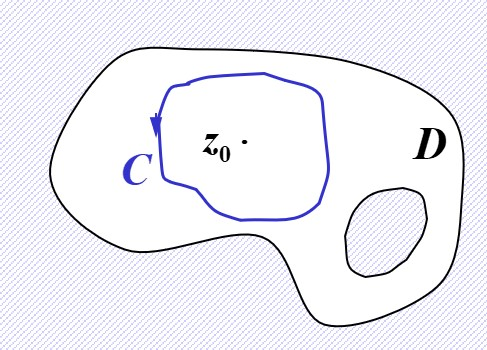
\includegraphics[width=\linewidth]{Figure_3_5_1.jpg}
      \end{figure}
    \end{minipage}
  \end{theorem}
\end{frame}

\begin{frame}
  \begin{proofs}
    Since $f(z)$ is continuous at $z_0$, when $\forall\varepsilon>0$,  $\exists\delta(\varepsilon)>0$, we have \\
    $|z-z_0|<\delta$, $|f(z)-f(z_0)|<\varepsilon$.\\
    Let K be a positive circle with center $z_0$  and radius $R(R<\delta)$, i.e., $K:|z-z_0|=R$. This circle $K$ is all inside $C$. We now have
    \begin{minipage}{0.6\linewidth}
      $\begin{aligned}
            & \oint_C \frac{f(z)}{z-z_0}\dif z=\oint_K \frac{f(z)}{z-z_0}\dif z        \\
          = & \oint_K \frac{f(z_0)}{z-z_0}\dif z+\oint_K \frac{f(z)-f(z_0)}{z-z_0}\dif z \\
          = & 2\pi if(z_0)+\oint_K \frac{f(z)-f(z_0)}{z-z_0}\dif z
        \end{aligned}$
    \end{minipage}\begin{minipage}{0.4\linewidth}
      \begin{figure}
        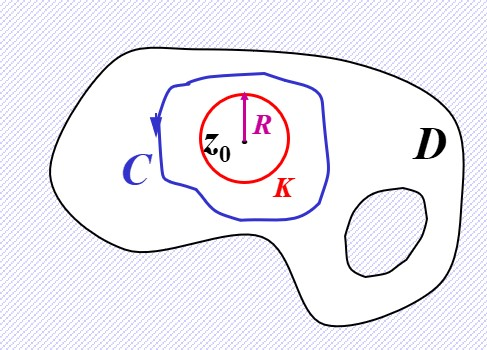
\includegraphics[width=\linewidth]{Figure_3_5_2.jpg}
      \end{figure}
    \end{minipage}
  \end{proofs}
\end{frame}

\begin{frame}
  \begin{proof}[\proofname\ (Cont.)]
    $\left|\oint_K \frac{f(z)-f(z_0)}{z-z_0}\dif z\right|\leq\oint_K \frac{|f(z)-f(z_0)|}{|z-z_0|}\dif s<\frac{\varepsilon}{R}\oint_K\dif s=2\pi\varepsilon.$\\
    The above inequality shows that the module of the left-hand integral is less than an arbitrarily small number, which gives  $\oint_K \frac{f(z)-f(z_0)}{z-z_0}\dif z=0$ .  \\

  \end{proof}
  {\color{blue}Cauchy's integral formula}: $f(z_0)=\frac{1}{2\pi i}\oint_C \frac{f(z)}{z-z_0}\dif z$
\end{frame}

\begin{frame}
  \begin{enumerate}
    \item []
          {\color{blue}Discussions about Cauchy's integral formula}:
          \begin{enumerate}[i)]
            \item The value of a function at any point $z_0$ in $C$ can be represented by its value on the boundary $C$. {\color{red}(another characteristic of analytic functions)}
            \item Cauchy's integral formula not only provides a method to calculate the integral of some complex functions along a closed path, but also gives an integral expression of analytical functions. {\color{red}(a powerful tool for studying analytic functions)}
            \item The value of an analytic function at the center of a circle is equal to its average value on the circumference.\\
                  For example, circle $C:z=z_0+Re^{i\theta}$,\\
                  $f(z_0)=\frac{1}{2\pi}\int_{0}^{2\pi}f(z_0+Re^{i\theta})\dif\theta$.
          \end{enumerate}
  \end{enumerate}
\end{frame}

\begin{frame}
  \begin{enumerate}
    \setcounter{enumi}{2}
    \item \textbf{Examples}
  \end{enumerate}
  \begin{example}
    Compute the integral $\oint_{|z|=2}\frac{e^z}{z-1}\dif z$.
  \end{example}
  \begin{solution}<2->
    Because $e^z$ is analytic in the complex plane and $z=1$ is inside  $|z|<2$,\\
    according to Cauchy's integral formula,\\
    $\oint_{|z|=2}\frac{e^z}{z-1}\dif z=2\pi i\cdot e^z\big|_{z=1}=2e\pi i$.
  \end{solution}
\end{frame}

\begin{frame}
  \begin{example}
    Compute the integral $\oint_{|z-i|=\frac{1}{2}}\frac{1}{z(z^2+1)}\dif z$.
  \end{example}
  \begin{solution}<2->
    $\frac{1}{z(z^2+1)}=\frac{1}{z(z+i)(z-i)}=\frac{\frac{1}{z(z+i)}}{z-i}$. $f(z)=\frac{1}{z(z+i)}$, $z_0=i$.\\
    Because $f(z)$ is analytic on and inside $|z-i|=\frac{1}{2}$, and $z_0=i$ is inside $|z-i|=\frac{1}{2}$, we have (according to Cauchy's integral formula) \\
    $\begin{aligned}
        \oint_{|z-i|=\frac{1}{2}}\frac{1}{z(z^2+1)}\dif z & =\oint_{|z-i|=\frac{1}{2}}\frac{\frac{1}{z(z+i)}}{z-i}\dif z \\
                                                          & =2\pi i\cdot\left.\frac{1}{z(z+i)}\right|_{z=i}             
                                                          & =2\pi i\cdot\frac{1}{2i^2}=-\pi i.
      \end{aligned}$
  \end{solution}
\end{frame}

\begin{frame}
  \begin{example}
    Let $C$ be the positively directed circle $x^2+y^2=3$ and $f(z)=\oint_C\frac{3\xi^2+7\xi+1}{\xi-z}\dif\xi$, find $f'(1+i)$.
  \end{example}
  \begin{solution}<2->
    \setlength{\baselineskip}{1.5\baselineskip}
    According to Cauchy's integral formula, when $z$ is in $C$,\\
    $f(z)=2\pi i\cdot(3\xi^2+7\xi+1)\big|_{\xi=z}=2\pi i(3z^2+7z+1)$.\\
    So $f'(z)=2\pi i(6z+7)$ and $1+i$ is in $C$,\\
    $f'(z+1)=2\pi(-6+13i)$.
  \end{solution}
\end{frame}

\begin{frame}
  \begin{example}
    Compute the integral $\oint_{C}\frac{\sin\frac{\pi}{4}}{z^2-1}\dif z$, where $C$ is
    \begin{minipage}{0.33\linewidth}
      \begin{enumerate}[1)]
        \item $|z+1|=\frac{1}{2}$;
      \end{enumerate}
    \end{minipage}\begin{minipage}{0.33\linewidth}
      \begin{enumerate}[2)]
        \item $|z-1|=\frac{1}{2}$;
      \end{enumerate}
    \end{minipage}\begin{minipage}{0.33\linewidth}
      \begin{enumerate}[3)]
        \setcounter{enumi}{2}
        \item $|z|=2$.
      \end{enumerate}
    \end{minipage}
  \end{example}
  \begin{solution}<2->
    \begin{enumerate}[1)]
      \item $\begin{aligned}[t]
                \oint_{|z+1|=\frac{1}{2}}\frac{\sin\frac{\pi}{4}}{z^2-1}\dif z & =\oint_{|z+1|=\frac{1}{2}}\frac{\frac{\sin\frac{\pi}{4}}{z-1}}{z+1}\dif z              \\
                                                                               & =2\pi i\cdot\left.\frac{\sin\frac{\pi}{4}}{z-1}\right|_{z=-1}=-\frac{\sqrt{2}}{2}\pi i;
              \end{aligned}$
    \end{enumerate}
  \end{solution}
\end{frame}

\begin{frame}
  \begin{solution}

    \begin{enumerate}[2)]

      \item $\begin{aligned}[t]
                \oint_{|z-1|=\frac{1}{2}}\frac{\sin\frac{\pi}{4}}{z^2-1}\dif z & =\oint_{|z-1|=\frac{1}{2}}\frac{\frac{\sin\frac{\pi}{4}}{z+1}}{z-1}\dif z             \\
                                                                               & =2\pi i\cdot\left.\frac{\sin\frac{\pi}{4}}{z+1}\right|_{z=1}=\frac{\sqrt{2}}{2}\pi i;
              \end{aligned}$
          \end{enumerate}
      \begin{enumerate}[3)]
      \item $\begin{aligned}[t]
                \oint_{|z|=2}\frac{\sin\frac{\pi}{4}}{z^2-1}\dif z & =\oint_{|z+1|=\frac{1}{2}}\frac{\frac{\sin\frac{\pi}{4}}{z+1}}{z-1}\dif z+\oint_{|z-1|=\frac{1}{2}}\frac{\frac{\sin\frac{\pi}{4}}{z+1}}{z-1}\dif z \\
                                                                   & =-\frac{\sqrt{2}}{2}\pi i+\frac{\sqrt{2}}{2}\pi i=0.
              \end{aligned}$
    \end{enumerate}
  \end{solution}
\end{frame}

\begin{frame}
  \begin{example}
    Compute the integral $\oint_{|z|=1}\frac{e^z}{z}\dif z$,\\ and prove $\int_o^\pi e^{\cos\theta}\cos(\sin\theta)\dif\theta=\pi$.
  \end{example}
  \begin{solution}<2->
    According to Cauchy's integral formula,\\
    $\oint_{|z|=1}\frac{e^z}{z}\dif z=2\pi i\cdot e^z\big|_{z=0}=2\pi i$.\\
    Let $z=re^{i\theta}\ (-\pi\leq\theta\leq\pi)$, $|z|=r=1$,
  \end{solution}
\end{frame}

\begin{frame}
  \begin{solution}
    $\begin{aligned}
        \oint_{|z|=1}\frac{e^z}{z}\dif z & =\int_{-\pi}^{\pi}\frac{e^{re^{i\theta}}}{re^{i\theta}}\cdot ire^{i\theta}\dif\theta=\int_{-\pi}^{\pi}ie^{e^{i\theta}}\dif\theta \\
                                         & =\int_{-\pi}^{\pi}ie^{e^{i\theta}}\dif\theta=\int_{-\pi}^{\pi}ie^{\cos\theta+i\sin\theta}\dif\theta                              \\
                                         & =2i\int_{0}^{\pi}e^{\cos\theta}\cos(\sin\theta)\dif\theta-i\underbrace {\int_{ - \pi }^\pi  {{e^{\cos \theta }}} \sin (\sin \theta )d\theta }_{ = 0}                                                     
      \end{aligned}$\\
    Since $\oint_{|z|=1}\frac{e^z}{z}\dif z=2\pi i$, and $\oint_{|z|=1}\frac{e^z}{z}\dif z=2i\int_{0}^{\pi}e^{\cos\theta}\cos(\sin\theta)\dif\theta$,\\
    we can compare the two equations to get $\int_{0}^{\pi}e^{\cos\theta}\cos(\sin\theta)\dif\theta=\pi$.
  \end{solution}
\end{frame}

\begin{frame}
  \begin{enumerate}
    \setcounter{enumi}{3}
    \item \textbf{Summary and Thinking}\\
          {\color{blue}Cauchy's integral formula}: $f(z_0)=\frac{1}{2\pi i}\oint_C \frac{f(z)}{z-z_0}\dif z$
  \end{enumerate}
\end{frame}

\section{Higher-order Derivatives}

\begin{frame}
	\frametitle{Outline}
	\tableofcontents[currentsection]
\end{frame}

\begin{frame}
	\begin{enumerate}
		\item \textbf{Main Theorems}
	\end{enumerate}
	\begin{theorem}
		The derivative of analytic function $f(z)$ is still analytic function, and its n-order derivative is
		\[f^{(n)}(z_0)=\frac{n!}{2\pi i}\oint_C \frac{f(z)}{(z-z_0)^{n+1}}\dif z,\ n=1,2,\cdots\]
		where $C$ is any positive simple closed curve who and whose inside are all contained in the analytic region $D$ of function $f(z)$, and $z_0$ is a point inside $C$.
	\end{theorem}
\end{frame}

\begin{frame}
	\begin{proofs}
		We consider the case of $n=1$ first, that is,
		\[f'(z_0)=\frac{1}{2\pi i}\oint_C \frac{f(z)}{(z-z_0)^2}\dif z.\]
		According to the definition of derivative,
		\[f'(z_0)=\lim_{\Delta z\to 0}\frac{f(z_0+\Delta z)-f(z_0)}{\Delta z}.\]
		According to Cauchy's integral formula
		\[f(z_0)=\frac{1}{2\pi i}\oint_c \frac{f(z)}{z-z_0}\dif z,\]
		\[f(z_0+\Delta z)=\frac{1}{2\pi i}\oint_c \frac{f(z)}{z-z_0-\Delta z}\dif z.\]
	\end{proofs}
\end{frame}

\begin{frame}
	\begin{proofs}[\proofname\ (Cont.)]
		Thus, we have
		\resizebox*{\linewidth}{!}{$\begin{aligned}
				&{{f({z_0} + \Delta z) - f({z_0})} \over {\Delta z}}{\rm{ }} = {1 \over {2\pi i\Delta z}}\left[ {\oint_c {{{f(z)} \over {z - {z_0} - \Delta z}}} dz - \oint_c {{{f(z)} \over {z - {z_0}}}} dz} \right] \\
				& =\frac{1}{2\pi i}\oint_c \frac{f(z)}{(z-z_0)(z-z_0-\Delta z)}\dif z                                              \\
				& =\frac{1}{2\pi i}\oint_c \frac{f(z)}{(z-z_0)^2}\dif z+{\color{blue}\begin{aligned}[t]
						\boxed{\color{black}\frac{1}{2\pi i}\oint_c \frac{\Delta zf(z)}{(z-z_0)^2(z-z_0-\Delta z)}\dif z} \\
						=I
				\end{aligned}}.
			\end{aligned}$}
		\begin{align*}
			|I| & =\frac{1}{2\pi}\left|\oint_c \frac{\Delta zf(z)}{(z-z_0)^2(z-z_0-\Delta z)}\dif z\right| \\
			& \leq\frac{1}{2\pi}\oint_c \frac{|\Delta z|\,|f(z)|}{|z-z_0|^2\,|z-z_0-\Delta z|}\dif z.
		\end{align*}
		Because $f(z)$ is analytic on $C$, $f(z)$ is continuous on $C$ and
	\end{proofs}
\end{frame}

\begin{frame}
	\begin{proofs}[\proofname\ (Cont.)]
		$f(z)$ is bounded on $C$. Then $\exists M>0$, such that $|f(z)\leq M|$.\\
		Let $d$ be the shortest distance from $z_0$ to all points on curve $C$, take $|\Delta z|$ small enough so that it satisfies $|\Delta z|<\frac{1}{2}d$, then\\
		\begin{minipage}{0.6\linewidth}
			\[|z-z_0|\geq d,\quad\frac{1}{|z-z_0|}\leq\frac{1}{d},\]
			\[|z-z_0-\Delta z|\geq|z-z_0|-|\Delta z|>\frac{d}{2},\]
			\[\frac{1}{|z-z_0-\Delta z|}<\frac{2}{d}\]
			% ,\quad |I|<|\Delta z|\frac{ML}{\pi d^3}
		\end{minipage}\begin{minipage}{0.4\linewidth}
			\begin{figure}
				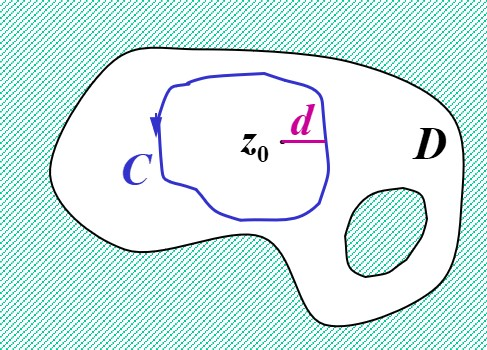
\includegraphics[width=\linewidth]{Figure_3_6_1.jpg}
			\end{figure}
		\end{minipage}\\
		\[\frac{|\Delta z|\,|f(z)|}{|z-z_0|^2\,|z-z_0-\Delta z|}\leq\frac{2}{d^3}|\Delta z|\,|f(z)|\]
	\end{proofs}
\end{frame}

\begin{frame}
	\begin{proofs}[\proofname\ (Cont.)]
		According to integral estimation inequality,
		\[|I|\leq\frac{|\Delta z|}{\pi d^3}\oint_C |f(z)|\dif s\leq|\Delta z|\frac{ML}{\pi d^3},\]
		where $L$ is the length of $C$. If $\Delta z\to 0$, $|I|\to 0$, then
		\[f'(z_0)=\lim_{\Delta z\to 0}\frac{f(z_0+\Delta z)-f(z_0)}{\Delta z}=\frac{1}{2\pi i}\oint_C \frac{f(z)}{(z-z_0)^2}\dif z.\]
		Reuse the above method to find $\lim_{\Delta z\to 0}\frac{f'(z_0+\Delta z)-f'(z_0)}{\Delta z}$,\\
		and get $f''(z_0)=\frac{2!}{2\pi i}\oint_C \frac{f(z)}{(z-z_0)^3}\dif z.$
	\end{proofs}
\end{frame}

\begin{frame}
	\begin{proof}[\proofname\ (Cont.)]
		By analogy, we can use mathematical induction to prove that
		\[f^{(n)}(z_0)=\frac{n!}{2\pi i}\oint_C \frac{f(z)}{(z-z_0)^{n+1}}\dif z.\]
	\end{proof}
	\color{blue}
	Cauchy's integral formula for derivatives is not to find the derivatives through integrals, but to find the integrals through derivatives.
\end{frame}

\begin{frame}
	\begin{enumerate}
		\setcounter{enumi}{1}
		\item \textbf{Examples}
	\end{enumerate}
	\begin{example}
		Compute the following integrals, where path $C:|z|=r>1$ is taken counterclockwise.\\
		\begin{minipage}{0.5\linewidth}
			\begin{enumerate}[1)]
				\item $\oint_C \frac{\cos\pi z}{(z-1)^5}\dif z$;
			\end{enumerate}
		\end{minipage}\begin{minipage}{0.5\linewidth}
			\begin{enumerate}[2)]
				\setcounter{enumi}{1}
				\item $\oint_C \frac{e^z}{(z^2+1)^2}\dif z$.
			\end{enumerate}
		\end{minipage}
	\end{example}
	\begin{solution}<2->
		\begin{enumerate}[1)]
			\item $\frac{\cos\pi z}{(z-1)^5}$ is not analytic at $z=1$ inside $C$,\\
			but $\cos\pi z$ is analytic on and inside $C$.\\
			According to Cauchy's integral formula for derivatives,\\
			$\oint_C \frac{\cos\pi z}{(z-1)^5}\dif z=\frac{2\pi i}{(5-1)!}(\cos\pi z)^{(4)}\big|_{z=1}=-\frac{\pi^5 i}{12}$.
		\end{enumerate}
	\end{solution}
\end{frame}

\begin{frame}
	\begin{solution}[Solution\ (Cont.)]
		\begin{enumerate}[2)]
			\setcounter{enumi}{1}
			\item $\frac{e^z}{(z^2+1)^2}$ is not analytic at $z=\pm i$ inside $C$.\\
			\begin{minipage}{0.62\linewidth}
				We make positive circles $C_1$ and $C_2$ with $z=\pm i$ as the center respectively in $C$.\\
				The function $\frac{e^z}{(z^2+1)^2}$ is analytic in the domain bounded by $C$, $C_1$ and $C_2$.
			\end{minipage}
			\
			\begin{minipage}{0.35\linewidth}
				\begin{figure}
					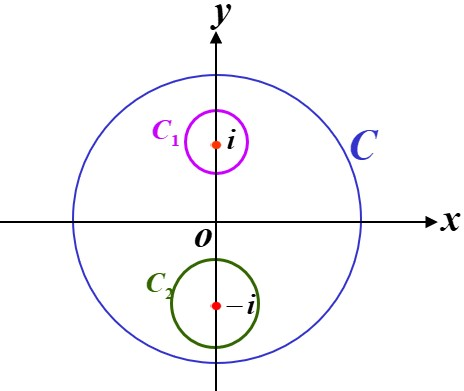
\includegraphics[width=\linewidth]{Figure_3_6_2.jpg}
				\end{figure}
			\end{minipage}
		\end{enumerate}
	\end{solution}
\end{frame}

\begin{frame}
	\begin{solution}[Solution\ (Cont.)]
		\begin{enumerate}
			\item []
			According to Cauchy's Theorem for multiply connected domains,\\
			$\oint_C \frac{e^z}{(z^2+1)^2}\dif z=\oint_{C_1} \frac{e^z}{(z^2+1)^2}\dif z+\oint_{C_2} \frac{e^z}{(z^2+1)^2}\dif z$.\\
			According to Cauchy's integral formula for derivatives,\\
			$\begin{aligned}
				\oint_{C_1} \frac{e^z}{(z^2+1)^2}\dif z & =\oint_{C_1} \frac{\frac{e^z}{(z+i)^2}}{(z-i)^2}\dif z                     \\
				& =\frac{2\pi i}{(2-1)!}\left.\left[\frac{e^z}{(z+i)^2}\right]'\right|_{z=i} \\
				& =\frac{(1-i)e^i}{2}\pi,
			\end{aligned}$
		\end{enumerate}
	\end{solution}
\end{frame}

\begin{frame}
	\begin{solution}[Solution\ (Cont.)]
		\begin{enumerate}
			\item []
			$\begin{aligned}
				\oint_{C_2} \frac{e^z}{(z^2+1)^2}\dif z & =\oint_{C_2} \frac{\frac{e^z}{(z-i)^2}}{(z+i)^2}\dif z                      \\
				& =\frac{2\pi i}{(2-1)!}\left.\left[\frac{e^z}{(z-i)^2}\right]'\right|_{z=-i} \\
				& =\frac{-(1+i)e^{-i}}{2}\pi.
			\end{aligned}$\\
			So, $\begin{aligned}[t]
				\oint_C \frac{e^z}{(z^2+1)^2}\dif z & =\frac{(1-i)e^i}{2}\pi+\frac{-(1+i)e^{-i}}{2}\pi \\
				& =\frac{\pi}{2}(1-i)(e^i-ie^{-i})                 \\
				& =\frac{\pi}{2}(1-i)^2(\cos 1-\sin 1)             \\
				& =i\pi\sqrt{2}\sin\left(1-\frac{\pi}{4}\right).
			\end{aligned}$
		\end{enumerate}
	\end{solution}
\end{frame}

\begin{frame}
	\begin{example}
		Compute the integral $\oint_C \frac{1}{(z-2)^2 z^3}\dif z$, where $C$ is:\\
		\begin{minipage}{0.5\linewidth}
			\begin{enumerate}[1)]
				\item $|z-3|=2$;
			\end{enumerate}
		\end{minipage}\begin{minipage}{0.5\linewidth}
			\begin{enumerate}[2)]
				\setcounter{enumi}{1}
				\item $|z-1|=3$.
			\end{enumerate}
		\end{minipage}
	\end{example}
	\begin{solution}<2->
		Function $\frac{1}{(z-2)^2 z^3}$ has two singularities $z=2$ and $z=0$.
		\begin{enumerate}[1)]
			\item Domain $|z-3|=2$ contains the singularity $z=2$.\\
			$\begin{aligned}
				\oint_C \frac{1}{(z-2)^2 z^3}\dif z & =\oint_C \frac{\frac{1}{z^3}}{(z-2)^2}\dif z                                        \\
				& =\frac{2\pi i}{1!}\left.\left(\frac{1}{z^3}\right)'\right|_{z=2}=-\frac{3\pi i}{8}.
			\end{aligned}$
		\end{enumerate}
	\end{solution}
\end{frame}

\begin{frame}
	\begin{solution}
		\begin{enumerate}[2)]
			\setcounter{enumi}{1}
			\item Domain $|z-3|=2$ contains the singularity $z=2$ and $z=0$.\\
			Make simple closed curves $C_1$ and $C_2$ contain $2$ and $0$ respectively, $C_1$ and $C_2$ do not contain each other and do not intersect each other.\\
			According to Cauchy's Theorem for multiply connected domains and Cauchy's integral formula for derivatives,\\
			$\begin{aligned}
				\oint_C \frac{1}{(z-2)^2 z^3}\dif z & =\oint_{C_1} \frac{1}{(z-2)^2 z^3}\dif z+\oint_{C_2} \frac{1}{(z-2)^2 z^3}\dif z                                                      \\
				& =\oint_{C_1} \frac{\frac{1}{(z-2)^2}}{z^3}\dif z+\oint_{C_2} \frac{\frac{1}{z^3}}{(z-2)^2}\dif z                                      \\
				& =\frac{2\pi i}{2!}\left.\left[\frac{1}{(z-2)^2}\right]''\right|_{z=0}+\frac{2\pi i}{1!}\left.\left(\frac{1}{z^3}\right)'\right|_{z=2} \\
				& =\frac{3\pi i}{8}-\frac{3\pi i}{8}=0.
			\end{aligned}$
		\end{enumerate}
	\end{solution}
\end{frame}

\begin{frame}
	\begin{example}[Morera's Theorem]
		Let $f(z)$ be a continuous function in a simply connected domain $B$ and suppose that the integral of $f(z)$ along any closed path lying entirely in $B$ is equal to zero. Prove that $f(z)$ is analytic in $B$.
	\end{example}
	\begin{proofs}<2->
		Let $z_0$ be a point in $B$, and $z$ be any point in $B$.\\
		The value of $\int_{z_0}^{z}f(\zeta)\dif\zeta$ is independent of the path that connects $z_0$ and $z$, and a single-valued function is defined as $F(z)=\int_{z_0}^{z}f(\zeta)\dif\zeta$.
	\end{proofs}
\end{frame}

\begin{frame}
	\begin{proof}[\proofname\ (Cont.)]
		\setlength{\baselineskip}{1.5\baselineskip}
		According to [Theorem 4.2], $F'(z)=f(z)$,\\
		$F(z)$ is an analytic function in $B$.\\
		Because the derivative of an analytic function is still an analytic function, $f(z)$ is an analytic function.
	\end{proof}
\end{frame}

\begin{frame}
	\begin{enumerate}
		\setcounter{enumi}{2}
		\item \textbf{Summary and Thinking}\\
		Cauchy's integral formula for derivatives is an important formula of complex integral. It shows the important conclusion that {\color{blue}the derivative of analytic function is still analytic function} and the essential difference between analytic function and real variable function.\\
		\color{blue}Cauchy's integral formula for derivatives:
		\[f^{(n)}(z_0)=\frac{n!}{2\pi i}\oint_C \frac{f(z)}{(z-z_0)^{n+1}}\dif z\]
	\end{enumerate}
\end{frame}

\begin{frame}
	\begin{example}
		What is the difference between the derivative of an analytic function and the derivative of a real function?
	\end{example}
	\begin{solution}<2->
		Cauchy's integral formula for derivatives shows that as long as the function $f(z)$ is differentiable everywhere in the closed region $D$, it must be infinitely differentiable, and its derivatives are all analytic functions on the closed region $D$.\\
		\color{red}This is fundamentally different from real variable functions.
	\end{solution}
\end{frame}

\begin{frame}
	\begin{example}
		How to compute the integral on a simple closed curve?
	\end{example}
\end{frame}

\section{Relations Between Analytic Functions and Harmonic Functions}

\begin{frame}
	\frametitle{Outline}
	\tableofcontents[currentsection]
\end{frame}

\begin{frame}
	\begin{enumerate}
		\item \textbf{Definition of Harmonic Functions}
	\end{enumerate}
	\begin{theorem}
		If the real bivariate function $\varphi(x,y)$ has second continuous partial derivatives in domain $D$ and satisfies Laplace's equation
		\[\frac{\partial^2 \varphi}{\partial x^2}+\frac{\partial^2 \varphi}{\partial y^2}=0,\]
		it is called a harmonic function in domain $D$.
	\end{theorem}
	\color{blue}
	Harmonic functions have very important applications in practical problems such as fluid mechanics and electromagnetic field theory.
\end{frame}

\begin{frame}
	\begin{enumerate}
		\setcounter{enumi}{1}
		\item \textbf{Relation Between Analytic Functions and Harmonic Functions}
		\begin{enumerate}[1)]
			\item Relations
		\end{enumerate}
	\end{enumerate}
	\begin{theorem}
		Any function that is analytic in domain $D$, its real and imaginary parts are harmonic functions in $D$.
	\end{theorem}
	\begin{proofs}
		Let $f(z)=u+iv$ be an analytic function in $D$, and it satisfies Cauchy-Riemann equations
		\[\frac{\partial u}{\partial x}=\frac{\partial v}{\partial y},\quad\frac{\partial u}{\partial y}=-\frac{\partial v}{\partial x}.\]
	\end{proofs}
\end{frame}

\begin{frame}
	\begin{proof}[\proofname\ (Cont.)]
		\[\frac{\partial^2 u}{\partial x^2}=\frac{\partial^2 v}{\partial y\partial x},\quad\frac{\partial^2 u}{\partial y^2}=-\frac{\partial^2 v}{\partial x\partial y}.\]
		According to Cauchy's integral formula for derivatives, $u$ and $v$ have continuous partial derivatives of any order, then
		\[\frac{\partial^2 v}{\partial y\partial x}=\frac{\partial^2 v}{\partial x\partial y}.\]
		\[\frac{\partial^2 u}{\partial x^2}+\frac{\partial^2 u}{\partial y^2}=0,\quad\frac{\partial^2 v}{\partial x^2}+\frac{\partial^2 v}{\partial y^2}=0.\]
		So $u$ and $v$ are harmonic functions.
	\end{proof}
\end{frame}

\begin{frame}
	\begin{enumerate}
		\item []
		\begin{enumerate}[1)]
			\setcounter{enumii}{1}
			\item Conjugate Harmonic Functions\\
			If $u(x,y)$ is the harmonic function given in domain $D$, we call the harmonic function $v(x,y)$ that makes $u+iv$ an analytic function in $D$ called the conjugate harmonic function of $u(x,y)$.\\
			It can be seen that if the two harmonic functions in $D$ satisfying the Cauchy-Riemann equations
			\[\frac{\partial u}{\partial x}=\frac{\partial v}{\partial y},\quad\frac{\partial u}{\partial y}=-\frac{\partial v}{\partial x},\]
			$v(x,y)$ is called the conjugate harmonic function of $u(x,y)$.\\
			\ \\
			\color{blue}
			The imaginary part of the analytic function in domain $D$ is the conjugate harmonic function of the real part.
		\end{enumerate}
	\end{enumerate}
\end{frame}

\begin{frame}
	\begin{enumerate}
		\item []
		\begin{enumerate}[1)]
			\setcounter{enumii}{2}
			\item 'Partial integral method'\\
			If a harmonic function $u(x,y)$ is known, then the Cauchy-Riemann equations can be used to find its conjugate harmonic function $v(x,y)$, thereby forming an analytic function $u+vi$. This method is called 'Partial integral method'.
		\end{enumerate}
	\end{enumerate}
	\begin{example}
		Prove $u(x,y)=y^3-3x^2y$ is a harmonic function, and determine its conjugate harmonic function $v(x,y)$ and the analytical function composed of them.
	\end{example}
\end{frame}

\begin{frame}
	\begin{solution}
		\[\frac{\partial u}{\partial x}=-6xy,\quad\frac{\partial^2 u}{\partial x^2}=-6y,\]
		\[\frac{\partial u}{\partial y}=3y^2-3x^2,\quad\frac{\partial^2 u}{\partial y^2}=6y.\]
		So $\frac{\partial^2 u}{\partial x^2}+\frac{\partial^2 u}{\partial y^2}=0$, $u(x,y)$ is a harmonic function.\\
		From $\frac{\partial v}{\partial y}=\frac{\partial u}{\partial x}=-6xy$,
		\[v(x,y)=-6\int xy\dif y=-3xy^2+g(x),\]
		\[\frac{\partial v}{\partial x}=-3y^2+g'(x).\]
	\end{solution}
\end{frame}

\begin{frame}
	\begin{solution}[Solution\ (Cont.)]
		From $\frac{\partial v}{\partial x}=-\frac{\partial u}{\partial y}=-3y^2+3x^2$,
		\[-3y^2+g'(x)=-3y^2+3x^2.\]
		So $g(x)=\int 3x^2\dif x=x^3+c$, $v(x,y)=x^3-3xy^2+c$.\\
		We get an analytic function $f(z)=u+iv=y^3-3x^2y+i\left(x^3-3xy^2+c\right)$,\\
		can also be written as $f(z)=i\left(z^3+c\right)$.
	\end{solution}
\end{frame}

\begin{frame}
	\begin{enumerate}
		\item []
		\begin{enumerate}[1)]
			\setcounter{enumii}{3}
			\item 'indefinite integral method'\\
			Given the harmonic function $u(x,y)$ or $v(x,y)$, the method of deriving the analytical function by indefinite integral is called 'indefinite integral method'.\\
			\ \\
			Implementation process of 'indefinite integral method':\\
			The derivative $f'(z)$ of the analytic function $f(z)=u+iv$ is still an analytic function,\\
			and $f'(z)=u_x+iv_x=u_x-iu_y=v_y+iv_x$.\\
		    Express $u_x-iu_y$ and $v_y+iv_x$ as functions of $z$,\\
			$f'(z)=u_x-iu_y=U(z)$, $f'(z)=v_y+iv_x=V(z)$.
		\end{enumerate}
	\end{enumerate}
\end{frame}

\begin{frame}
	
	\begin{enumerate}
		\item []
		\begin{enumerate}
			\item []
			Integrate the above two equations to obtain:\\
			\begin{minipage}{0.5\linewidth}
				\color{blue}
				$\boxed{\color{black}f(z)=\int U(z)\dif z+c}$\color{black},\\
				\color{blue}
				Find $f(z)$ with known\\
				real part $u$
			\end{minipage}\begin{minipage}{0.5\linewidth}
				\color{red}
				$\boxed{\color{black}f(z)=\int V(z)\dif z+c}$\color{black}.\\
				\color{red}
				Find $f(z)$ with known\\
				imaginary part $v$
			\end{minipage}
		\end{enumerate}
	\end{enumerate}
\end{frame}

\begin{frame}
	\begin{example}
		Determine the analytic function $f(z)$ in [Example 7.1] by 'indefinite integral method', where its real part is $u(x,y)=y^3-3x^2y$.
	\end{example}
	\begin{solution}<2->
		$\begin{aligned}
			f'(z) & =U(z)=u_x-iu_y=-6xy-i\left(3y^2-3x^2\right) \\
			& =3i\left(x^2+2xyi-y^2\right)=3iz^2,
		\end{aligned}$\\
		$f(z)=\int 3iz^2\dif z=iz^3+c_1$,\\
		(Because the real part of $f(z)$ is known, it is impossible to contain any real constants, the constant $c_1$ is any pure imaginary number.)\\
		So, $f(z)=i\left(z^3+c\right)$.
	\end{solution}
\end{frame}


%\begin{frame}
%	\begin{example}
%		Determine the analytic function $f(z)$ in [Example 7.1] by 'curve integral method', where its real part is $u(x,y)=y^3-3x^2y$.
%	\end{example}
%	\begin{solution}<2->
%		$\begin{aligned}
%			\dif v & =v_x\dif x+v_y\dif y=-u_y\dif x+u_x\dif y \\
%			& =-\left(3y^2-3x^2\right)\dif x-6xy\dif y,
%		\end{aligned}$\\
%		$\begin{aligned}
%			v(x,y) & =\int_{(0,0)}^{(x,y)}-\left(3y^2-3x^2\right)\dif x-6xy\dif y \\
%			& =\int_0^x 3x^2\dif x+\int_0^y -6xy\dif y=x^3-3xy^2,
%		\end{aligned}$\\
%		$f(z)=y^3-3x^2y+i\left(x^3-3xy^2+c\right)=i\left(z^3+c\right)$.
%	\end{solution}
%\end{frame}

\begin{frame}
	\begin{example}
		Determine the analytic function $f(z)=u+iv$, where $u+v=(x-y)\left(x^2+4xy+y^2\right)-2(x+y)$.
	\end{example}
	\begin{solution}<2->
		Differentiating both sides of the equation,\\
		$u_x+v_x=\left(x^2+4xy+y^2\right)+(x-y)(2x+4y)-2$,\\
		$u_y+v_y=-\left(x^2+4xy+y^2\right)+(x-y)(2x+4y)-2$,\\
		and $\frac{\partial u}{\partial x}=\frac{\partial v}{\partial y}$, $\frac{\partial u}{\partial y}=-\frac{\partial v}{\partial x}$.
	\end{solution}
\end{frame}

\begin{frame}
	\begin{solution}[Solution\ (Cont.)]
		So add and subtract the above two equations respectively to get\\
		$v_y=3x^2-3y^2-2$, $v_x=6xy$,\\
		$\begin{aligned}
			f'(z) & =v_y+iv_x=3x^2-3y^2-2+6xyi \\
			& =3z^2-2,
		\end{aligned}$\\
		$f(z)=\int \left(3z^2-2\right)\dif z=z^3-2z+c$.
	\end{solution}
\end{frame}

\begin{frame}
	\begin{enumerate}
		\setcounter{enumi}{2}
		\item \textbf{Summary and Thinking}\\
		In this section, we learn the concept of harmonic function, the relationship between analytic function and harmonic function, and the concept of conjugate harmonic function.\\
		\ \\
		Note:
		\begin{enumerate}[1)]
			\item The complex function $u+iv$ formed by any two harmonic functions $u$ and $v$ does not have to be an analytic function.
			\item The $v$ that satisfies the Cauchy-Riemann equations $u_x=v_y$, $v_x=-u_y$, is called the conjugate harmonic function of $u$. Note that the order of $u$ and $v$ cannot be reversed.
		\end{enumerate}
	\end{enumerate}
\end{frame}

\end{document}
